\documentclass[10pt, oneside]{article}
\usepackage[letterpaper, margin=1in]{geometry}
%\usepackage[parfill]{parskip}    		% Activate to begin paragraphs with an empty line rather than an indent
\usepackage{graphicx}
\usepackage{amssymb}
\usepackage[style=numeric,firstinits=true,backend=bibtex]{biblatex}
\addbibresource{references}
\usepackage{wrapfig}
\usepackage{algorithm}
\usepackage{algpseudocode}
\usepackage{amsmath}
\usepackage{amsfonts}
\usepackage{listings}
\usepackage{url}
\usepackage{tikz}
\usetikzlibrary{calc,shapes.multipart,chains,arrows}
\usepackage{graphicx}
\usepackage{nameref}
\usepackage{xspace}
\usepackage{adjustbox}
\usepackage{framed}
\usepackage[all]{xy}
\usepackage{txfonts,pxfonts}
\usepackage{bm}
\usepackage{enumerate}
\usepackage{algorithm}
\usepackage{subfigure}
\usepackage{algpseudocode}
\usepackage[english,printdayoff]{isodate}
\usepackage[pdftitle={PhD Written Qualifier Exam - Simone Atzeni}, pdfauthor={Simone
  Atzeni}, pdfsubject={PhD Written Qualifier}]{hyperref}

\title{\textbf{PhD Written Qualifier Exam}\\{\normalsize Examiners: Ganesh Gopalakrishnan,
Zvonimir Rakamari\'c, Hari Sundar, Ryan Stutsman}}
%
\author{Simone Atzeni\\{\small simone@cs.utah.edu}}
%
\date{January 18, 2015 -- January 25, 2015}

\newcommand{\rfuz}{\textsc{RaceFuzzer}\xspace}
\newcommand{\archer}{\textsc{Archer}\xspace}
\newcommand{\symp}{\textsc{Symple}\xspace}
\renewcommand*{\bibfont}{\footnotesize}
\lstset{basicstyle=\ttfamily,
escapeinside={||},
mathescape=true}

\newenvironment{blockquote}{\par\medskip\leftskip=4em\rightskip=2em\noindent\ignorespaces}{\par\medskip}

\begin{document}
\maketitle
\newpage
\setcounter{tocdepth}{1}
\tableofcontents
\newpage

% This paper by Raychev describes parallelizing user-defined aggregations
% using Symbolic Execution

% http://research.microsoft.com/pubs/256579/143-raychev.pdf

% Describe the ideas in this paper and see if these ideas could be used for
% OpenMP race detection (inability to parallelize = race). If not, why not, or
% in which cases? Could this help your research in any way?

\begin{refsection}
\section{Questions from Ganesh Gopalakrishnan}
\label{sec:member1}

\subsection{Describe the ideas in this paper\dots}
\label{sec:member11}

The authors in~\cite{Raychev:2015:PUA:2815400.2815418} present a system,
called \symp, that allows a user to automatically parallelize and perform
User-defined aggregations (UDAs) queries, in order to optimize and exploit the
parallelism available in large-scale data-processing systems, such as
MapReduce and Hadoop.
%

\begin{wrapfigure}{l}{0.23\textwidth}
  \centering
  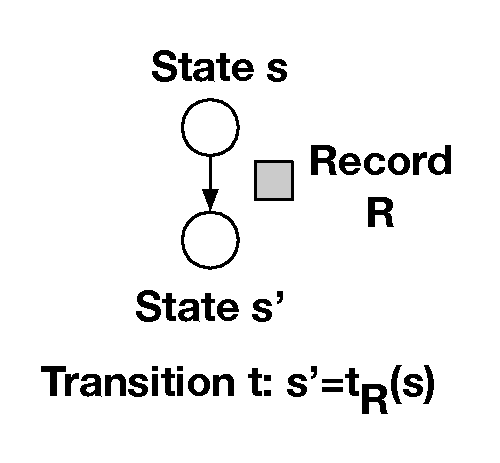
\includegraphics[width=0.23\textwidth]{figures/symple_ex1}
  \caption{Transition on a record $R$ from state $s$ to the next state $s'$.}
  \label{fig:symple_ex1}
\end{wrapfigure}

\noindent
These big systems, in general, provide parallel support for aggregation
functions, such as \emph{Max}, \emph{Count}, \emph{Sum}, since they are easy
to parallelize and allow to obtain high performance.
%
However, complex aggregation queries, such as UDAs, are hard to parallelize
because of their data dependencies (i.e.\ loop-carried data dependency), so
the execution has to be run sequentially introducing a slowdown of several
orders-of-magnitude.
%
For example, if we have a big amount of data (records) that come from the logs
of an e-commerce website and we want to query the \emph{number of reviews per
  user session}, it would be non-trivial to parallelize.
%
\symp provides a mechanism for performing
MapReduce-style~\cite{Dean:2008:MSD:1327452.1327492} aggregate functions,
processing chunks of the divided input in parallel, and running a symbolic
execution of the UDAs where those dependencies are treated as ``unknown''
symbolic values.
%
As a result, the symbolic execution returns a \emph{symbolic summary} which is
basically the output of the UDA as a function of its input.
%
\symp can run in parallel the symbolic executions on each input chunk and
compose the summaries in a final reduction step to produce the result that
would match a sequential execution of the UDA.
\\

\noindent
\paragraph{Symbolic parallelism in detail:}

A given UDA query, that has to be computed by the system, is expressed in a
dialect of C++.
%
The values of variables used by the function for the computation are called
the \emph{State s}.

\begin{wrapfigure}{r}{0.20\textwidth}
  \centering
  \vspace{-15pt}
  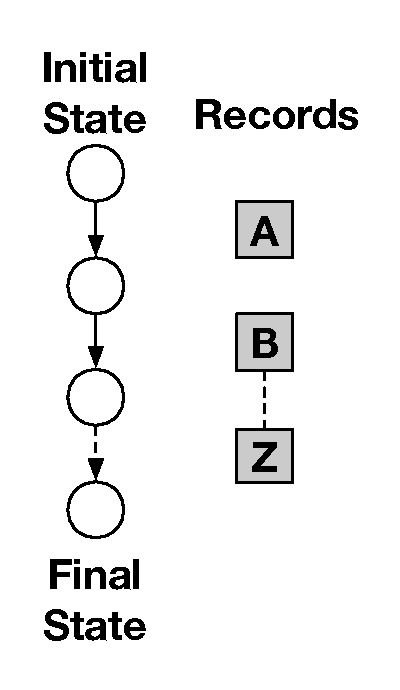
\includegraphics[width=0.18\textwidth]{figures/symple_ex2}
  \vspace{-10pt}
  \caption{Sequential execution of the query on the entire dataset.}
  \label{fig:symple_ex2}
\end{wrapfigure}

\noindent
The operations executed by the query on the records, for example to find the
\emph{number of reviews per user session} (referring to the previous example),
might change the state of the computation, these operations are the
\emph{transitions}.
%
Therefore, a transition for a record \emph{R} changes the current state from
\emph{s} to the next state \emph{s'} as shown in Figure~\ref{fig:symple_ex1}.
%
As stated above, when we have a complex query, it is hard to parallelize
because the next state that the query has to compute always depends on the
previous state, so data dependencies are the real problem.
%
In a sequential execution (Figure~\ref{fig:symple_ex2}), it would not be a
problem since each transition is computed sequentially by only one process.

In order to parallelize such a query using symbolic execution (or
\emph{symbolic parallelism}), \symp proceeds in the following way.
%
Once the input is divided in chunks, the symbolic parallelism mechanism
computes the query \textbf{concretely} on the first chunk, obtaining the state
\textbf{s} as shown in Figure~\ref{fig:symple_ex3}.
%
Now, the symbolic parallelism can execute symbolically, and in parallel the
query on all the other chunks.
%
It means that for each record, in a given chunk, the symbolic execution
applies the transitions starting from a symbolic unknown state \textbf{x}.
%
Figure~\ref{fig:symple_ex4} shows how this computation returns a function
\textbf{F} of $x$, where the transition has been applied on the records $D$,
$E$, and $F$.
%
Finally, we combine the function $F$ on the concrete state $s$ and we obtain
the final state, which would be the result of $F(s) = t_D(t_E(t_F(s)))$.

% \begin{figure}
%   \begin{minipage}[b]{0.3\textwidth}
%     \begin{flushleft}
%       \raisebox{30pt}{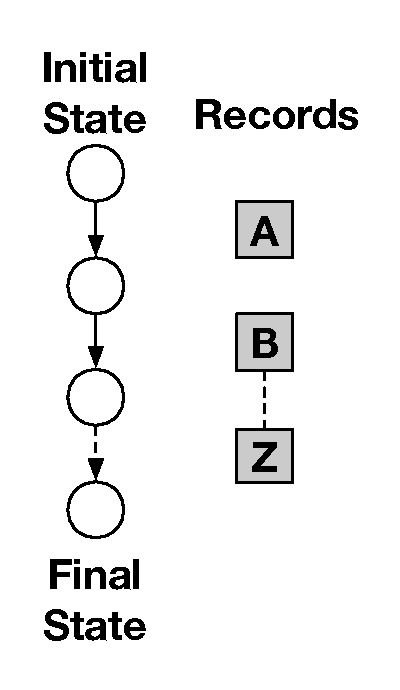
\includegraphics[width=0.6\textwidth]{figures/symple_ex2}}
%       \caption{Sequential execution of the query on the entire dataset.}
%       \label{fig:symple_ex2}
%     \end{flushleft}
%   \end{minipage}
%   \hfill
%   \begin{minipage}[b]{0.3\textwidth}
%     \centering
%     \raisebox{35pt}{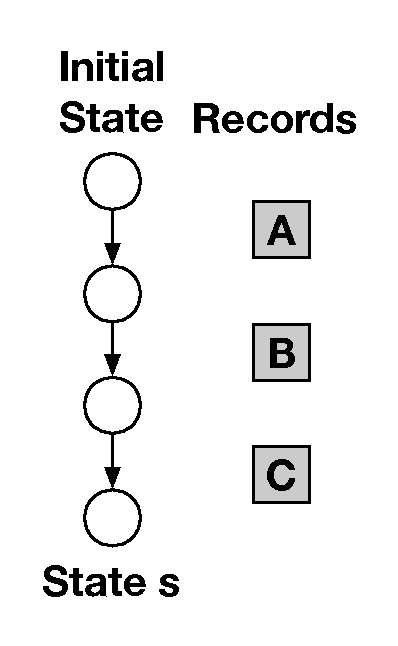
\includegraphics[width=0.65\textwidth]{figures/symple_ex3}}
%     \caption{Concrete execution of the query on the first chunk of data.}
%     \label{fig:symple_ex3}
%   \end{minipage}
%   \hfill
%   \begin{minipage}[b]{0.3\textwidth}
%     \begin{flushright}
%       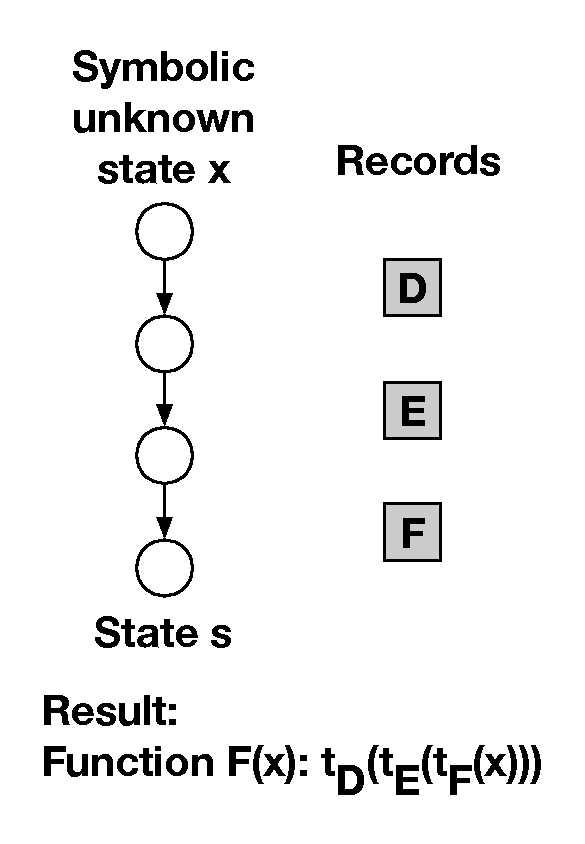
\includegraphics[width=0.8\textwidth]{figures/symple_ex4}
%       \caption{Parallel symbolic execution on the rest of the data chunks.}
%       \label{fig:symple_ex4}
%     \end{flushright}
%   \end{minipage}
% \end{figure}

% \begin{figure}
%   \begin{minipage}[b]{0.3\textwidth}
%     \begin{flushleft}
%       \centering
%       \raisebox{35pt}{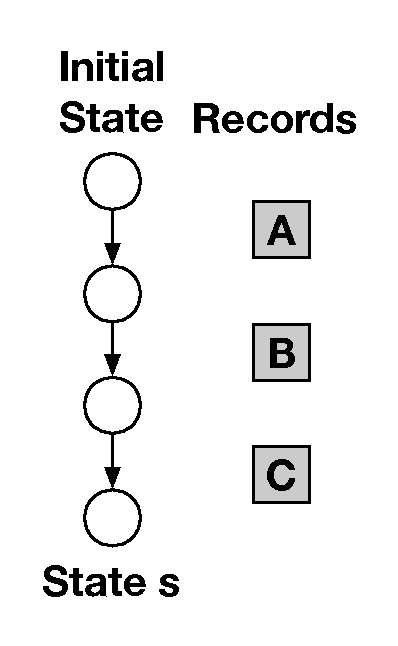
\includegraphics[width=0.65\textwidth]{figures/symple_ex3}}
%       \caption{Concrete execution of the query on the first chunk of data.}
%       \label{fig:symple_ex3}
%     \end{flushleft}
%   \end{minipage}
%   \hfill
%   \begin{minipage}[b]{0.3\textwidth}
%     \centering
%     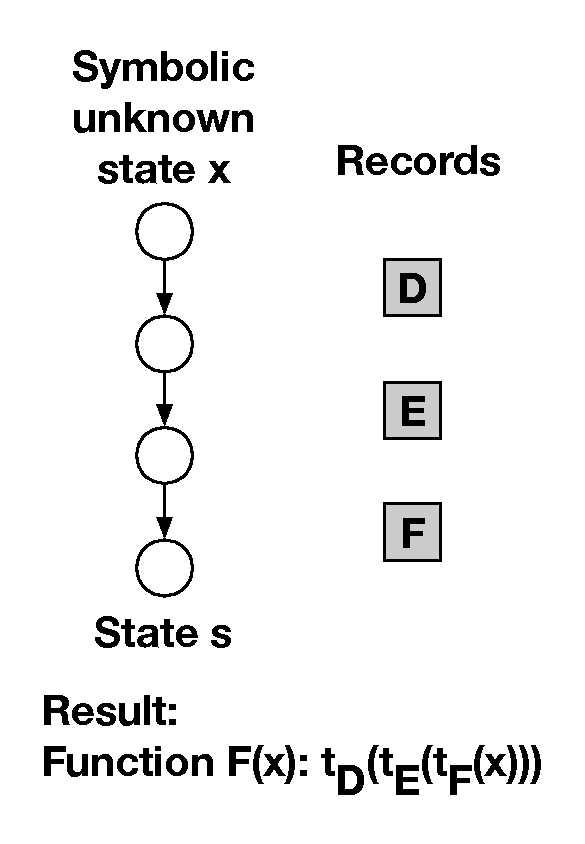
\includegraphics[width=0.8\textwidth]{figures/symple_ex4}
%     \caption{Parallel symbolic execution on the rest of the data chunks.}
%     \label{fig:symple_ex4}
%   \end{minipage}
%   \hfill
%   \begin{minipage}[b]{0.3\textwidth}
%     \begin{flushright}
%       \centering
%       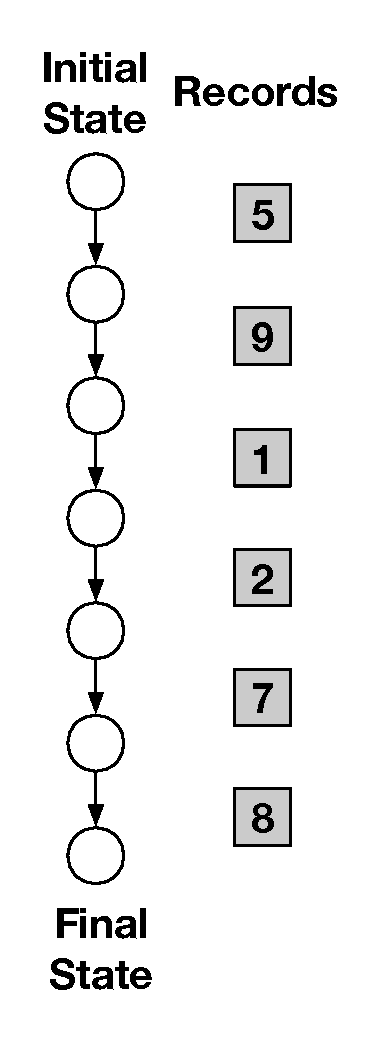
\includegraphics[width=0.6\textwidth]{figures/symple_ex5}
%       \caption{Parallel symbolic execution on the rest of the data chunks.}
%       \label{fig:symple_ex5}
%     \end{flushright}
%   \end{minipage}
% \end{figure}

\begin{figure}
  \begin{minipage}[b]{0.3\textwidth}
    \begin{flushleft}
      \centering
      \raisebox{0pt}{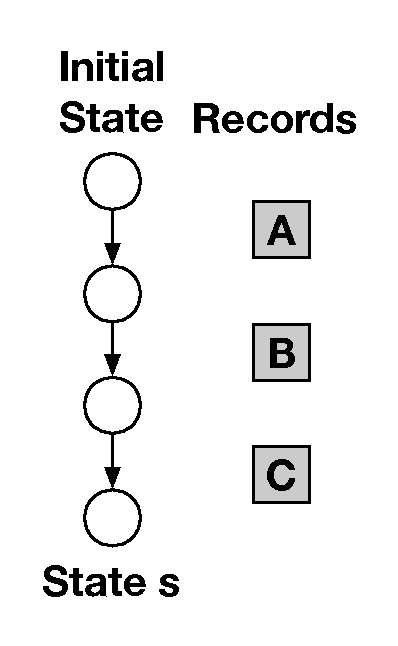
\includegraphics[width=0.6\textwidth]{figures/symple_ex3}}
      \caption{Concrete execution of the query on the first chunk of data.}
      \label{fig:symple_ex3}
    \end{flushleft}
  \end{minipage}
  \hfill
  \begin{minipage}[b]{0.3\textwidth}
    \centering
    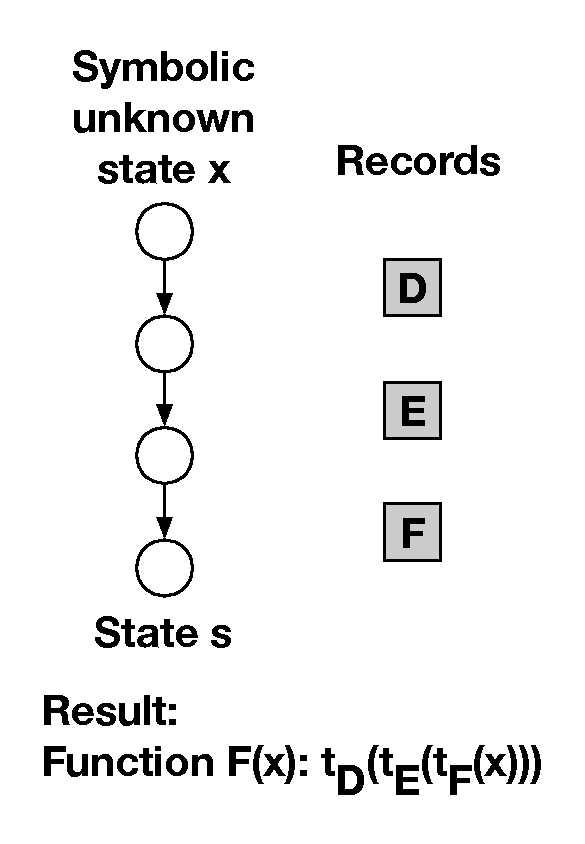
\includegraphics[width=0.8\textwidth]{figures/symple_ex4}
    \caption{Parallel symbolic execution on the rest of the data chunks.}
    \label{fig:symple_ex4}
  \end{minipage}
  \hfill
  \begin{minipage}[b]{0.3\textwidth}
    \begin{flushright}
      \centering
      \raisebox{0pt}{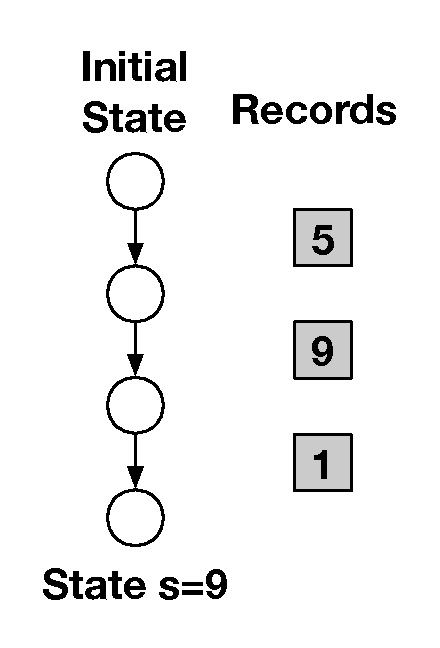
\includegraphics[width=0.6\textwidth]{figures/symple_ex6}}
      \caption{Concrete execution of the query on the first chunk of data.}
      \label{fig:symple_ex6}
    \end{flushright}
  \end{minipage}
\end{figure}

\paragraph*{Example:}
Let us now apply the symbolic parallelism on a real example.
%
Suppose we want to compute the aggregation function $Max$ defined as:

\begin{center}
  \begin{lstlisting}
    if |\textbf{state}| < |\textbf{{\color{blue}value}}| then |\textbf{state}| = |{\textbf{\color{blue}value}}|
  \end{lstlisting}
\end{center}

\noindent
on a list of integers such as $\{5, 9, 1, 2, 7, 8\}$, and divide the integers
into two chunks: $\{5, 9, 1\}$ and $\{2, 7, 8\}$.
%
The computation on the first chunk will execute concretely, so the max value
will be $9$ (Figure~\ref{fig:symple_ex6}).
%
In the meantime, in parallel, the symbolic execution performs the computation
on the second chunk starting from an unknown symbolic state $x$.
%
As shown in Figure~\ref{fig:symple_ex7}, the symbolic execution is executed on
each value of the second chunk and it returns $F$ as a function of $x$.
%
Now, the function $F$ can be combined with the concrete value computed on the
first chunk and the final state will be $F(9)=9$.

Figure~\ref{fig:symple_ex8} shows a complete symbolic pipeline of the same
aggregation function \emph{Max} on the input $\{1, 8, 3, 4, 7, 6, 9, 5, 2\}$.
%
The first step is to split the data in chunks and assign each one of them to a
different task.
%
The second step runs the symbolic executions in parallel (notice that the
first task is always computed concretely).
%
$Task 1$ and $Task 2$ return two functions that are going to be combined with
the initial state computed by $Task 0$.
%
Indeed, the max value computed by $Task 0$, which is $8$ will be used in place
of $x$ in the function returned by $Task 1$.
%
Then, the new value obtained by the first combination will be used with the
function returned by $Task 2$, and the max value computed.

%  \begin{figure}
%   \begin{minipage}[b]{0.4\textwidth}
%     \begin{flushleft}
%       \centering
%       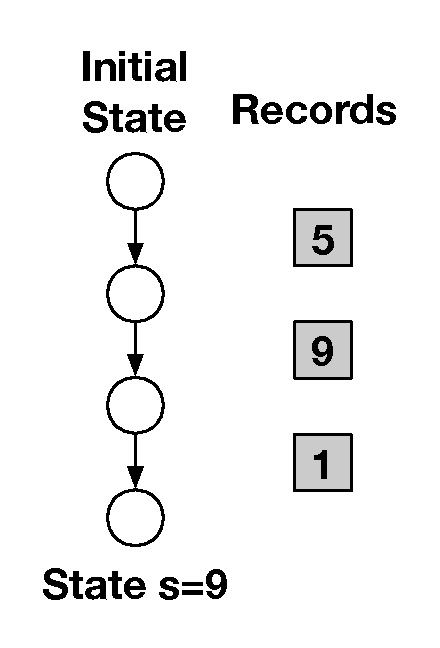
\includegraphics[scale=0.7]{figures/symple_ex6}
%       \caption{Concrete execution of the query on the first chunk of data.}
%       \label{fig:symple_ex6}
%     \end{flushleft}
%   \end{minipage}
%   \hfill
%   \begin{minipage}[b]{0.55\textwidth}
%     \begin{flushright}
%       \centering
%       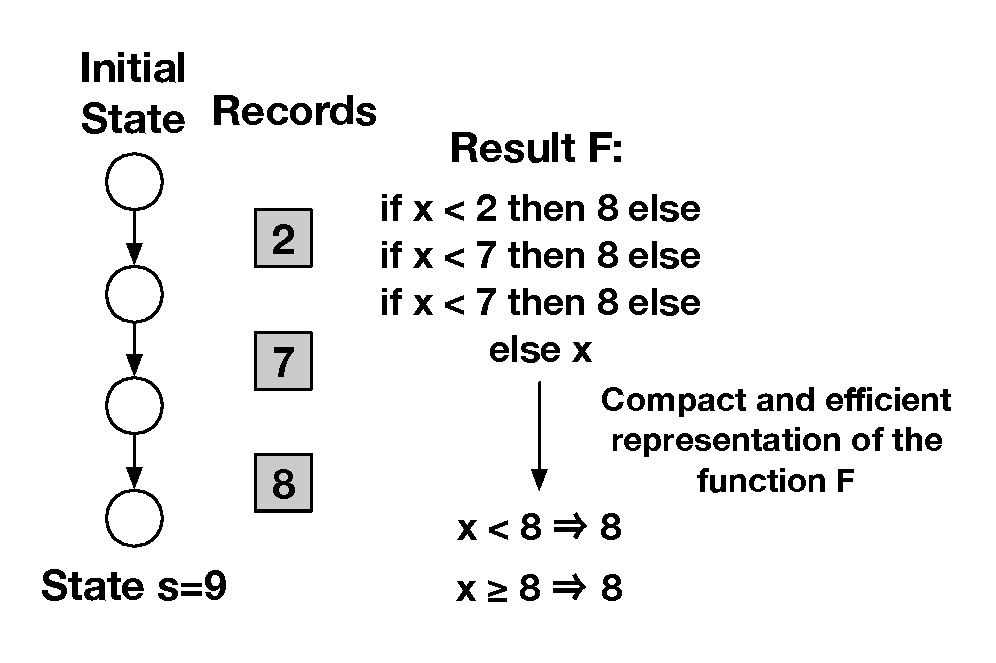
\includegraphics[scale=0.7]{figures/symple_ex7}
%       \caption{Parallel symbolic execution on the rest of the data chunks.}
%       \label{fig:symple_ex7}
%     \end{flushright}
%   \end{minipage}
% \end{figure}

 \begin{figure}[H]
  \begin{minipage}[b]{0.47\textwidth}
    \begin{flushleft}
      \centering
      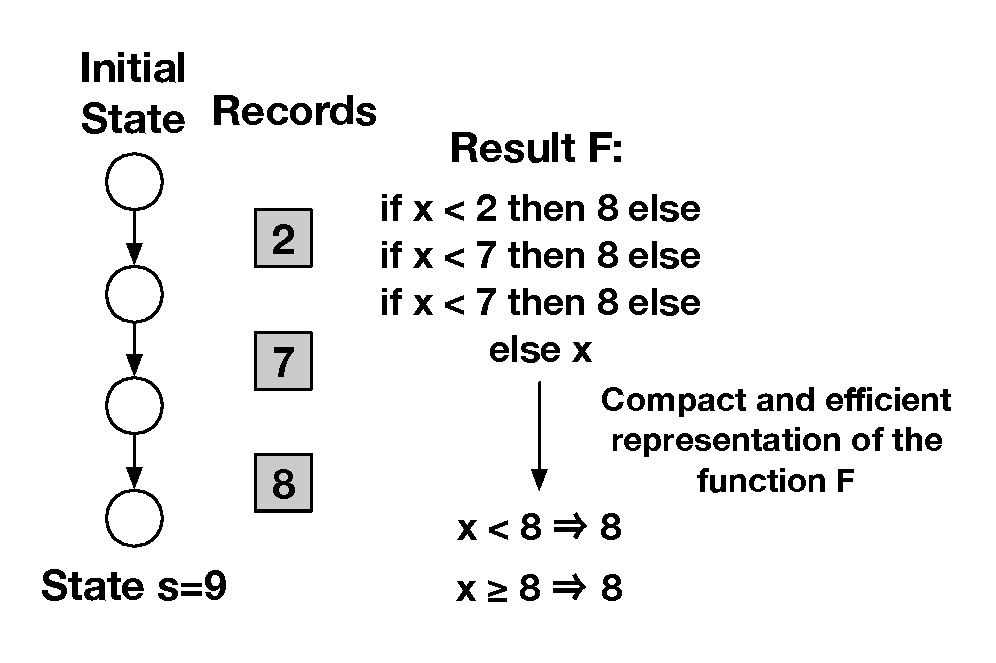
\includegraphics[scale=0.5]{figures/symple_ex7}
      \caption{Parallel symbolic execution on the rest of the data chunks.}
      \label{fig:symple_ex7}
    \end{flushleft}
  \end{minipage}
  \hfill
  \begin{minipage}[b]{0.47\textwidth}
    \begin{flushleft}
      \centering
      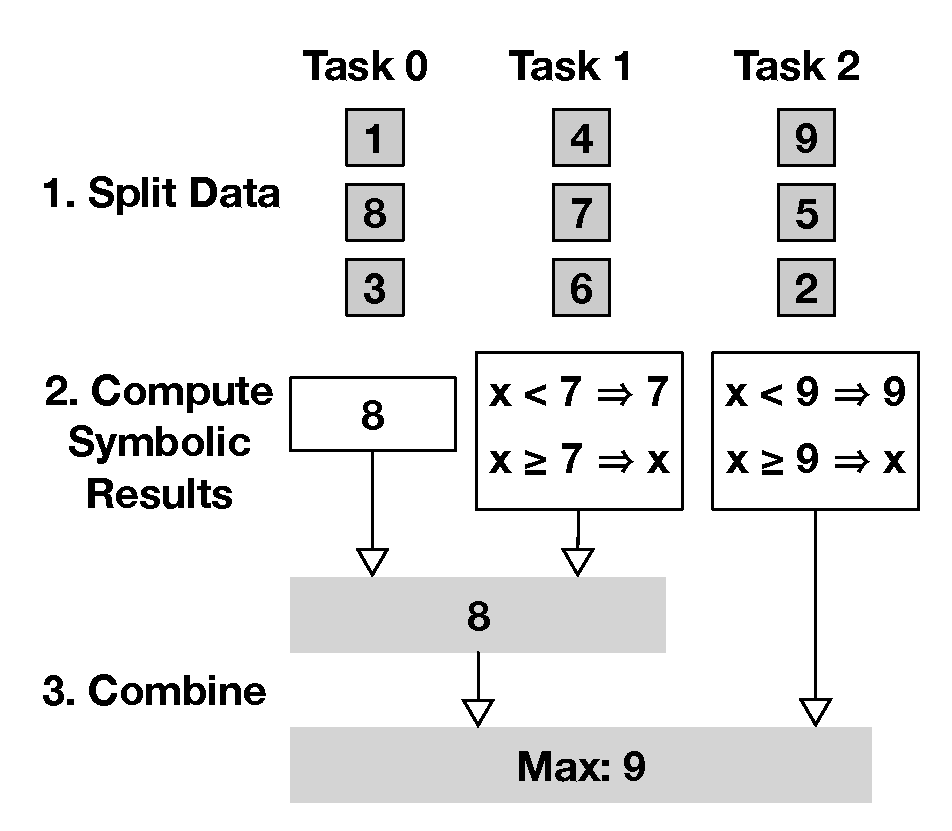
\includegraphics[scale=0.5]{figures/symple_ex8}
      \caption{Full parallel symbolic execution
        pipeline. \textcolor{white}{empty}}
      \label{fig:symple_ex8}
    \end{flushleft}
  \end{minipage}
\end{figure}

% \begin{figure}
%   \centering
%   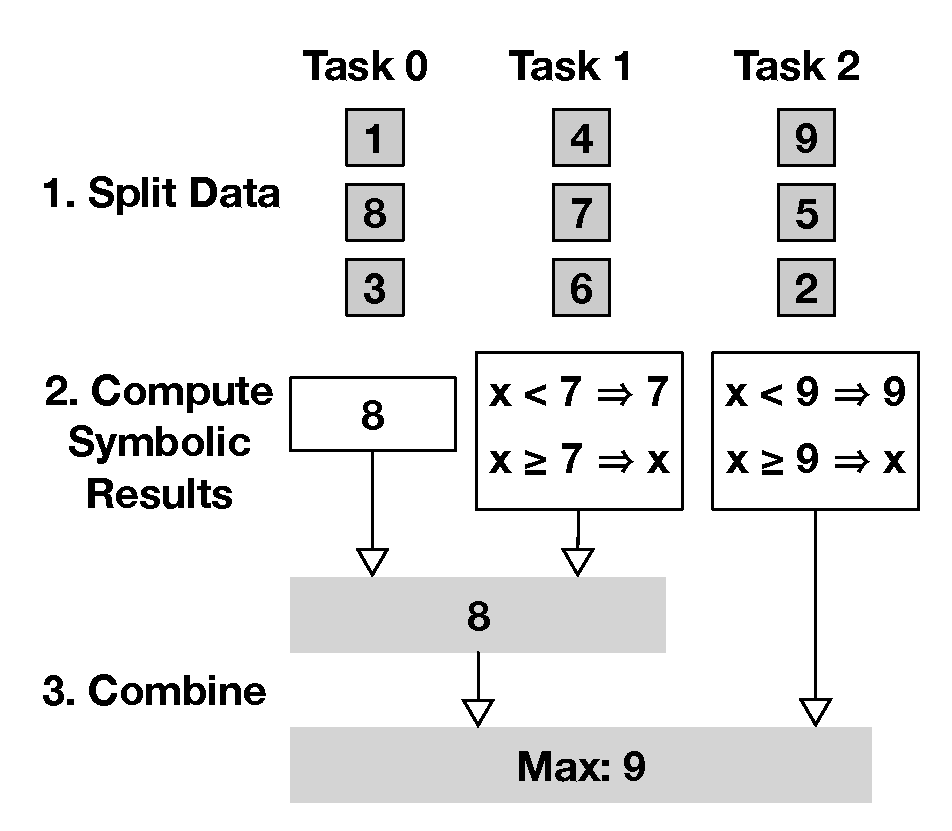
\includegraphics[scale=0.7]{figures/symple_ex8}
%   \caption{Full parallel symbolic execution pipeline.}
%   \label{fig:symple_ex8}
% \end{figure}

\paragraph{Discussion:} In the example of Figure~\ref{fig:symple_ex6} the
symbolic execution computes a function for each value in the data set.
%
This function is actually the result of the symbolic execution as it explores
all the possible paths (i.e.\ of the computation of the query) and accumulates
the path constraints for each decision (as shown in Figure~3
in~\cite{Raychev:2015:PUA:2815400.2815418}).
%
A path constraint implies a function: for instance if the symbolic execution
is computing the aggregation function $Max$ and it is on a state $x$, when it
encounters a value $v$ from the input, it will generate two path constraints
``$x < v \implies max = v$'' and ``$x \geq v \implies max = x$''.
%
The main point in the function generation is its shape, because it influences
the performance of the entire computation.
%
Indeed, \symp introduces its own data types (which look and behave like
standard C++ types) that are the key to control the shape of the functions.

The equivalent of the C++ data type \emph{int} in \symp is called symbolic
integer \emph{SymInt}.
%
The \emph{SymInt} data type has a very specific shape:

\begin{equation*}
x \in [l, u] \implies ax+b
\end{equation*}

This means that if the value of the integer $x$ is in the interval $[l,u]$ the
resulting function is of the form $ax+b$.
%
The \emph{SymInt} data type stores the four constants $l, u, a, b$, that allow
to keep the function always in the shape $ax+b$, and defines transformers to
maintain the function shape.
%
For example:

\begin{itemize}
\item If the state \emph{s} is a concrete value $b$, we have $x \in [l, u] \implies 0x+b$.
\item If the state \emph{s} is a symbolic value $x$, we have $x \in [l, u] \ \implies 1x+0$.
\item If $s = 7$, $x \in [l, u] \implies 0x + 7$.
\item If $(s \leq 5)$, $x \in [l, 5] \implies ax + b$.
\end{itemize}

There are other data types that follow the same idea, such as \emph{SymBool},
\emph{SymEnum}, \emph{SymVector}, and \emph{SymPredicate}. Furthermore \symp
allow the user to define custom data structures through composition of data
types.

\subsection{\dots~and see if these ideas could be used
  for OpenMP race detection (inability to parallelize = race).
  %
  If not, why not, or in which cases?
  %
  Could this help your research in any way?}
\label{sec:member12}

In OpenMP a data race may happen when the programmer parallelizes, with some
of the OpenMP construct, a portion of code (i.e.\ loop) that carries a data
dependency.
%
The compiler does not perform any check on the OpenMP code, therefore if the
developer parallelizes a for-loop like that one in Figure~\ref{fig:race1}, the
compilation result will be a program that might be racy when executed with
multiple threads.
%
\begin{wrapfigure}{R}{0.35\textwidth}
\begin{lstlisting}[language=C]
  #pragma omp parallel for
  for (i = 1; i < N; i++)
     sum = sum + a[i];
\end{lstlisting}
\caption{OpenMP sum parallel reduction loop with a data race on the variable
  $sum$, because of a data dependency and lack of synchronization.}
\label{fig:race1}
\end{wrapfigure}
%
The example in Figure~\ref{fig:race1} performs a reduction of a sum operation,
and has a race condition on the variable $sum$.
%
% Most likely, the example in Figure~\ref{fig:race1}, if executed with two or
% more threads, will manifest a race condition in some of the array locations.
%
Due to the data dependency and the absence of any synchronization mechanism,
two different threads will be allowed to access the location of $sum$
simultaneously, generating the data race.

The system \symp handles the $sum$ reduction by splitting the input for the
function in chunks, and running in parallel the symbolic execution on each
input chunk to compute the intermediate summaries.
%
The results from each symbolic execution will then be combined together to
generate the final result, as seen previously in the description of the
algorithm.
%
The \symp approach does not perform any checks on the aggregation operation,
so basically it does not know if the function has any data dependency or not.
%
The system always performs symbolic execution, even in absence of data
dependency (which would allow it to run in parallel without symbolic
execution).

The authors in the paper do not clarify if the system runs a data dependency
analysis to discover possible data dependencies (and so potential races),
before parallelizing the query.
%
I suspect that, no matter if the function carries some data dependecies or
not, \symp will always run symbolic parallelism.
%
If there are no data dependencies, after a certain number of steps the
symbolic representation will become equivalent to the concrete so it would not
be an issue.
%
On the other hand this approach, in presence of data-dependency-free
functions, introduces some overheads, as there would be a better way to
parallelize.

I believe the symbolic approach of \symp could not be used for my OpenMP data
race detection research.
%
While \symp tries to find an efficient way to parallelize complex UDAs, in
OpenMP programs the code is already parallelized by the programmer, and it
requires some techniques (static or dynamic) to analyze it in order to find
any data races.
%
However, the parallel symbolic executions approach may be useful in improving
existing techniques for data race detection.

The \emph{happens-before} relation is a well-known technique to find,
precisely, data races on threaded programs at runtime~\cite{Flanagan:2009}.
%
On the other hand, it only finds races on branches of the program that are
actually executed, and it also demands many resources, and generates high
runtime and memory overheads.
%
A symbolic execution approach could improve both problems of this dynamic
technique:

\begin{enumerate}
\item \emph{Explore multiple path of the program:} The symbolic execution
  might run the OpenMP program symbolically, generating symbolic memory
  locations (that a thread would access at runtime), executing the program
  operations, and when present the synchronization operations.
  %
  Therefore, the input for a \emph{symbolic happens-before} would be:

  \begin{itemize}
  \item Threads info (i.e. TID)
  \item The ``symbolic addresses'' (per thread).
  \item Per-thread and per-lock vector clocks and/or epochs; updated during
    the symbolic execution of the synchronization operations.
  \item The type of the operations executed (i.e.\ read or write).
  \end{itemize}

  If the relation is not satisfied, which means:
  %
  \begin{blockquote}
    \emph{a symbolic memory location exists, it has been accessed
    by two different threads, at least one of the thread operation is a
    write, and an order of the two events can not be established,}
  \end{blockquote}
  %
  a race is detected and reported.

  In the case of branches, the symbolic execution (i.e.\ based on the data
  types) could generate and explore different paths of the OpenMP program
  spotting more racy behaviors.
\item \emph{Reducing runtime and memory overhead:} The parallel programming
  model of OpenMP is very structured, in the sense that during an execution of
  a program, the OpenMP runtime:
  \begin{enumerate}
  \item Spawns a team of threads when it encounters a parallel section.
  \item Executes the work in parallel.
  \item Destroys the threads team when the parallel section terminates.
  \item The program continues the execution sequentially until the following
    parallel section.
  \end{enumerate}
  %
  This would allow to distribute, across multiple processes (i.e.\ in a
  cluster), the symbolic execution of different parallel sections, while the
  single symbolic execution is itself already parallel and distributed across
  multiple cores.
  %
  An approach like this could mitigate the runtime and memory overhead
  generated by the happens-before technique, and the additional overhead which
  may arise from the multiple paths explored by the symbolic execution.
\end{enumerate}

\printbibliography

\end{refsection}

%%% Local Variables:
%%% mode: latex
%%% eval: (flyspell-mode 1)
%%% TeX-master: "root.tex"
%%% End:

% Thoroughly study the following paper by Koushik Sen on using dynamic testing
% to establish whether an alarm is a real data race or not: K. Sen, "Race
% Directed Random Testing of Concurrent Programs," in Proc. ACM SIGPLAN
% Conference on Programming Language Design and Implementation (PLDI'08),
% 2008, pp. 11-21.  http://srl.cs.berkeley.edu/~ksen/papers/raced.pdf

% Describe in detail the technique introduced in this paper. Make sure to
% critically assess its pros and cons. In addition, connect this work to your
% own research. Could you envision it being used in your own work on OpenMP
% data race detection? If so, then describe how. If not, then clarify why
% not. Your response should be roughly 3-4 pages long. Good luck.

\begin{refsection}
\section{Questions from Zvonimir Rakamari\'c}
\label{sec:member2}

\textbf{Describe in detail the technique introduced
  in~\cite{Sen:2008:RDR:1375581.1375584}.
  %
  Make sure to critically assess its pros and cons.
  %
  In addition, connect this work to your own research.
  %
  Could you envision it being used in your own work on OpenMP data race
  detection?
  %
  If so, then describe how.
  %
  If not, then clarify why not.}

\vspace{10pt}
\noindent
In the paper~\cite{Sen:2008:RDR:1375581.1375584} the author proposes a
technique to establish whether a reported race in a concurrent program is
harmful or not.
%
This technique is called \emph{race--directed random testing} or \rfuz.
%
A harmful race is defined as a race that could lead to errors or exceptions
in the programs (i.e.\ crash) such as run-time errors or programmer defined
assertions.
%
Finding these bugs caused by data races is hard.
%
Existing techniques are either imprecise (e.g.\ static, dynamic and hybrid
race detectors), and reported bugs require manual inspection to determine
whether they are real races or just false alarms.
%
On the contrary, precise techniques cannot predict potential races that could
happen in other paths of the program (e.g.\ happens-before based
detectors~\cite{Flanagan:2009}).
\\

\noindent
The \rfuz technique consists of two phases:

\paragraph{Phase 1 - Hybrid-Race Detection:}
The phase~1 of the algorithm is quite simple, the tool the author implemented
uses an existing hybrid race detection
technique~\cite{O'Callahan:2003:HDD:781498.781528}, which combines
lockset-based detection and happens-before-based detection to identify and
create a set of potential races in a program.
%
Each race in the set is identified as a pair of concurrent statements, called
\emph{racing pair of statements}, that can potentially race during a
concurrent execution.

From the paper:

\noindent\rule[0.5ex]{\linewidth}{1pt}

At runtime the race detection algorithm checks, for each pair of events
$<e_i,e_j>$, the following conditions:

\begin{enumerate}
\item
  $e_i = MEM(\sigma_i, m_i, a_i, t_i, L_i) \wedge e_j = MEM(\sigma_j, m_j,
  a_j, t_j, L_j)$,
  where $MEM(\sigma, m, a, t, L)$ denotes that a thread $t$ performs an access
  $a$ (read or write) to a memory location $m$ while holding the set of locks
  $L$ and executing the statement $\sigma$;
\item $t_i \neq t_j$, the two events are performed by two different
  threads;
\item $m_i = m_j$, the two events access the same memory location;
\item $a_i = WRITE \vee a_j = WRITE$, at least one of the memory accesses is a
  write;
\item \label{itm:lockset} $L_i \cap L_j = \emptyset$, the two events are not holding a common lock;
\item $\neg(e_i \prec e_j) \wedge \neg(e_j \prec e_i)$, one of the events (and
  so the memory accesses) does not happens-before the other (i.e.\ they are
  concurrent).
\end{enumerate}

If these conditions hold, then $(\sigma_i, \sigma_j)$ is a racing pair of
statements.
%
All the detected racing pairs will form the $RaceSet$ that will be used by the
phase~2 of the \rfuz.

\noindent\rule[0.5ex]{\linewidth}{1pt}

Phase~1 applies a hybrid race detection
technique~\cite{O'Callahan:2003:HDD:781498.781528} that combines the lock-set
detection and the happens-before approaches.
%
The hybrid technique essentially merges the lockset detection check
(condition~\ref{itm:lockset}) and a limited happens-before detection check.
%
The happens-before approach reports real races, and they are a subset of the
races reported by lockset-based detection, as stated by Theorem~1
in~\cite{O'Callahan:2003:HDD:781498.781528}.
%
Some of the details are intentionally omitted in order to focus on the novel
contribution of \rfuz which is discussed the phase~2.

\paragraph{Phase 2 - \rfuz:}
The phase~2 is the core of the \rfuz algorithm.
%
\rfuz will try to determine if each racing pair in the $RaceSet$ will actually
race in a real concurrent execution~\footnote{Due to imprecisions of the
  hybrid-race detection technique it might not actually race.}.
%
\rfuz re-executes the program with a random schedule for each pair in the set
of potential race.
%
The random scheduling execution increases the probability for \rfuz to find
harmful races, as it can enforce a certain order between two statements.
%
This is different to normal random testing which may always propose always the
same order of statements.
%
% \rfuz will try to determine if each racing pair of statements
% $(\sigma_i, \sigma_j) \in RaceSet$ will actually race in a real concurrent
% execution~\footnote{Due to imprecision of the hybrid-race detection technique
%   it might not actually race}.
% %
% \rfuz re-executes the program with a random schedule for each pair in the set
% of potential race $<\sigma_1,\sigma_2>$ (with $<\sigma_1,\sigma_2>$ the pair
% of concurrent statements).
% %
% During the execution \rfuz picks a random thread at each program state.
% %
% When the thread next-statement $ns_1$ is in $<\sigma_1,\sigma_2>$, postpone
% its execution.
% %
% \rfuz picks another thread and check if next-statement $ns_2$ is in
% $<\sigma_1,\sigma_2>$ and forms a race with $ns_1$~\footnote{Two statements
%   race when they are executed by two different threads, both access the same
%   memory location, and at least one of the statement is a write.}.
% %
% If this happens, \rfuz has found a real race formed by $<ns_1,ns_2>$.
% %
% When \rfuz reports a race, in order to continue the algorithm, it executes
% randomly one of the racing statements and keeps to postpone the execution of the
% other one.
%
% The random scheduling execution increases the probability for \rfuz to find
% harmful races, because it can enforce a certain order between two statements,
% differently than a normal random testing that may propose always the same
% order of statements.
%
% (for example in Figure~1
% of~\cite{Sen:2008:RDR:1375581.1375584} a false race would be reported by
% a hybrid-race detection technique while there is no race since the two
% instructions order is ensured by data)
\\

\noindent
Before going into the details of the \rfuz algorithm, let us consider the
following definitions:

\begin{itemize}
\item $Enabled(s)$ indicates the set of threads that are enabled in the
  program state $s$.
\item $Alive(s)$ indicates the set of threads that are still running and have
  not yet reached the state $s$.
\item $Execute(s,t)$ returns the state reached by executing the next statement
  of thread $t$ in state $s$.
\item $NextStmt(s,t)$ indicates the next statement that thread $t$ would
  execute in state $s$.
\item $Racing(s,t,postponed)$ returns the thread $t' \in postponed$ such that
  the statements that $t$ and $t'$ are about to execute (respectively
  $NextStmt(s,t)$ and $NextStmt(s,t')$) access the same memory location and at
  least one of the accesses is a write (race).
\end{itemize}

\noindent
Therefore, given in input the initial state of the program $s_0$ and the
$RaceSet$, the \rfuz algorithm (Algorithm~1 in
\cite{Sen:2008:RDR:1375581.1375584}) for a given racing pair performs the
following steps:

\begin{itemize}
\item Initialize the current program state $s$ to $s_0$.
\item Initialize an empty set to keep the statements where execution will be
  postponed ($postponed = \emptyset$).
\item As long as there are $Enabled$ threads in the current state $s$, \rfuz
  will keep executing the following steps:
  \begin{enumerate}
  \item Pick a random thread $t$ from $Enabled(s)$ that are not in the
    $postponed$ set (this assures to pick a different thread every time).
  \item Whenever a thread is about to execute one of the racing statements
    ($NextStmt(s,t) \in RaceSet$) the scheduler \emph{postpones} it
    ($postponed := postponed \cup {t}$).
  \item The execution remains postponed, until a different other thread also
    tries to execute one of the racing statements: if the two statements
    access the same memory location and one of them is a write, \rfuz has
    found a race ($Racing(s,t,postponed) \neq \emptyset$).
  \item Report the real race, and randomly resolve it, which consists of
    executing one of the statements (and keep postponing the other) to check
    if something bad can happen.
    %
    The execution of one random statement will also generate the next state of
    the program for the continuation of the algorithm ($s := Execute(s,t)$).
  \end{enumerate}
\end{itemize}

\noindent
Particular cases:

\begin{itemize}
\item It may happen that all threads are postponed because, even though they
  are trying to execute a racing statement, none of them actually race as they
  access different shared memory locations.
  %
  The racing pair are the result of an imprecise hybrid race detection
  technique, which may report pairs that do not result in an actual race.
  %
  This situation turns into a deadlock in the \rfuz algorithm, that the
  scheduler breaks randomly by picking one of the threads from the $postponed$
  set.
\item \rfuz algorithm keeps looping until there are not $Enabled$
  threads. When it reaches this condition, if there are still active threads
  ($(Active(s) \neq \emptyset$) we have a deadlock in the concurrent program.
\end{itemize}

\subsection*{\rfuz case study}
\label{sec:member21}

The example in Figure~1 of~\cite{Sen:2008:RDR:1375581.1375584} is an
interesting case study which compares \rfuz with a pure
happens-before-based technique.
%
The program shows two threads that access three global variables $x, y, z$,
and according to a hybrid race detection technique, they race in two cases: on
variable $x$ and on variable $z$.
%
\rfuz will be invoked several times with different random seeds (to generate
different thread schedulings) on the $RaceSet=\{1, 10\}$ and on the
$RaceSet=\{5,7\}$.

\paragraph{Case 1:} $RaceSet=\{1, 10\}$. In case $thread1$ first reaches
statement $1$ it will be postponed.
%
Since $y == 0$, $thread2$ will never reach statement $10$ and will terminate,
therefore no real race will be reported.
%
The other schedule is likely to reach statement $10$ first, and as this is not
possible due to the initialization of the variables, no race will again be
reported.

\paragraph{Case 2:} $RaceSet=\{5, 7\}$. If $thread1$ reaches statement $5$
first, it is postponed until $thread2$ reaches statement $7$.
%
In this case \rfuz reports a real race since both statements access the same
memory location and one of them ($7$) is a write.
%
The same scenario happens if $thread2$ reaches first statement $7$.

\subparagraph{Discussion on Case1:} At the end of the first paragraph of
Section~2.2 of the paper, the author specifies that, even though the tool that
implements \rfuz uses hybrid race detection, any static or dynamic race
detection technique could be used.
%
The author claims that, in the Case~1 of the previous example, hybrid race
detection technique will always report a race over the variable $x$, however
this might not be true if the tool would use a pure happens-before relation.
%
In the example in Figure~1 of~\cite{Sen:2008:RDR:1375581.1375584} the only
schedule that would allow a hybrid technique to report the race on $x$ is the
one reported in Figure~\ref{fig:execution1}, where \emph{Thread~1} is executed
before \emph{Thread~2}, however this would not be the case for the
happens-before-based techniques.
%
All the other schedules would not allow \emph{Thread~2} to reach variable $x$
because of $y \neq 1$, so no technique would report a race.

Figure~\ref{fig:omprace1} shows indeed how the happens-before relation, based
on the schedule in Table~\ref{fig:execution1}, would not report the race on
$x$.
%
(Note that in this case I am not considering $z$ since it does not play an
important role).
%
Let us use DJIT+~\cite{Pozniansky:2007:MEO:1228965.1228969, Flanagan:2009} as
the algorithm that implements the happens-before in Figure~\ref{fig:omprace1}.
%
When $T2$ performs the last read on variable $x$, DJIT+ compares $T2$'s Vector
Clock (VC) with the write's VC for $x$.
%
DJIT+ applies the rule in Algorithm~\ref{alg:djit}.
%
$\mathbb{W}_x(t)$ ($<1, 0>$) and $\mathbb{C}_t(t)$ ($<1, 1>$) have the same
clock for \emph{Thread~1} and the clock for \emph{Thread~2} is smaller in the
write's vector clock of $x$, this satisfy the previous rule and no race is
reported.
%
In this particular case \rfuz does not perform better than an
happens-before-based technique, since Phase~1 alone would be able to give an
exact answer of the races in the program~\footnote{The race in Case~2 would be
  reported by both hybrid technique or happens-before alone.}.
\\

\noindent
Instead, the second example in Figure~2
of~\cite{Sen:2008:RDR:1375581.1375584}, shows a better scenario where the
happens-before relation would miss the race on variable $x$ with a default or
a simple random scheduler.
%
\rfuz in this case would allow to explore several schedules and create the
right scenario to detect and resolve the race condition.
%
Indeed, in Phase~1 the hybrid race detection will detect the pair of racing
statements $(8, 10)$.
%
In Phase~2, \rfuz will randomly pick one of the threads: if it picks $thread1$
the algorithm will first postpone the statement $8$, otherwise if it picks
$thread2$ the statement $10$ will be postponed.
%
In either case, \rfuz will report the race.

\begin{figure}
  \begin{minipage}[b]{0.28\textwidth}
    \centering
    \begin{algorithm}[H]
      \caption{DJIT+ Read rule}
      \label{alg:djit}
      \begin{algorithmic}
        \If {$\mathbb{R}_x(t) \neq \mathbb{C}_t(t)$}

        \texttt{assert} $\mathbb{W}_x \sqsubseteq \mathbb{C}_t$

        $\mathbb{R}_x(t) := \mathbb{C}_t(t)$
        \EndIf
      \end{algorithmic}
    \end{algorithm}
    \phantom{1}
    \phantom{2}
    \phantom{3}
    \phantom{4}
    \begin{tabular}{c c}
      Thread~1 & Thread~2 \\
      \hline
      w(x)   & \\
      acq(L) & \\
      w(y)   & \\
      rel(L) & \\
               & acq(L) \\
               & r(y) \\
               & r(x) \\
               & rel(L) \\
      \hline
    \end{tabular}
    \caption{Events Trace of example in Figure~1 in~\cite{Sen:2008:RDR:1375581.1375584}}
    \label{fig:execution1}
  \end{minipage}
  \hfill
  \begin{minipage}[b]{0.7\textwidth}
    \framebox[1.0\width]{
      \resizebox{1.0\textwidth}{!}{
        \xymatrix@C=0.5em@R=1.2em{
          \mathbf{T1} & & \mathbf{T2} & & \mathbf{L_L} & & \mathbf{R_x} & & \mathbf{W_x} & & \mathbf{R_y} & & \mathbf{W_y} \\
          <1, 0> \ar[d]^{w(x)} & & <0, 1> & & <0, 0> & & <0, 0> & & <0, 0> & & <0, 0> & & <0, 0> \\
          <1, 0> \ar[d]^{acq(L)} & & <0, 1> & & <0, 0> \ar@{-->}[lllld] & & <0, 0> & & <1, 0> & & <0, 0> & & <0, 0> \\
          <1, 0> \ar[d]^{w(y)} & & <0, 1> & & <0, 0> & & <0, 0> & & <1, 0> & & <0, 0> & & <0, 0> \\
          <1, 0> \ar[d]^{rel(L)} \ar@{-->}[rrrrd] & & <0, 1>  & & <0, 0> & & <0, 0> & & <1, 0> & & <0, 0> & & <1, 0> \\
          <2, 0> & & <0, 1> \ar[d]^{acq(L)} & & <1, 0> \ar@{-->}[lld] & & <0, 0> & & <1, 0> & & <0, 0> & & <1, 0> \\
          <2, 0> & & <1, 1> \ar[d]^{r(y)} & & <1, 0> & & <0, 0> & & <1, 0> & & <0, 0> & & <1, 0> \\
          <2, 0> & & <1, 1> \ar[d]^{r(x)} & & <1, 0> & & <0, 0> & & <1, 0> \ar@{-->}[lllllddd] & & <0, 1> & & <1, 0> \\
          & & <1, 1> \ar@{-->}[rdd] & & & & & & & & & & \\
          \\
          & & & W_x \sqsubseteq C_t \ar[d] & & & & & & & & &\\
          & & & \textbf{NO RACE} & & & & & & & & & }}
    }
    \caption{Race detection applying
      DJIT+~\cite{Pozniansky:2007:MEO:1228965.1228969} algorithm based on
      happens-before relation and vector clock, on example in Figure~\ref{fig:execution1}.}
    \label{fig:omprace1}
  \end{minipage}
  \vspace{-10pt}
\end{figure}

% \subsubsection*{Example 2}
% The example in Figure~2 of~\cite{Sen:2008:RDR:1375581.1375584} shows
% another example of two threads that access a global variable $x$.
% %
% The access on $x$ by the two threads will clearly results in a data race
% because of lack of synchronization.
% %
% Indeed, a hybrid data race detection technique will predict the race between
% statement $8$ and $10$.
% %
% However, because of the structure of the program, a happens-before-based
% detection techniques may not be able to report the race with high probability.
% %
% Indeed, this probability would depend on the scheduling of the two threads, a
% simple randomized scheduler would not execute the racing statement temporally
% next to each other and the happens-before relation would miss this race.
% %
% This example

\subsection*{Pros and Cons of \rfuz}
\label{sec:member22}

\rfuz differs from classical race detection techniques as it is able to
distinguish whether a race is harmful (or not), by executing potential racing
statements.
%
This is an important feature when used to distinguish real races from false
alarms reported by hybrid techniques.
%
However, the author claims that an advantage of \rfuz is that it separates
harmful races from benign races.
%
In my opinion, the benign races should still be reported as harmful races.
%
Whilst \rfuz may identify a race as benign, it is important to keep in mind
that a ``benign'' race in a debugging environment become harmful in production
because of compilers optimization, often omitted in the development phase.
%
As studied by Boehm~\cite{Boehm:2011:MPB:2001252.2001255}, compilers assume
race free code and apply transformations that, in presence of a ``benign''
race, might results in harmful races~\cite{ec2_2015-agralslpm}.
%
\rfuz also identifies those races that do not generate any program exception as
``benign''.
%
This is a major downside of the algorithm, since this category includes the
races that might produce wrong results (i.e.\ bad non-determinism~\footnote{I
  call it ``bad non-determinism'' to distinguish it from other types of
  non-determinism such as the one caused by the order in floating-point
  operations that it is in general expected and sometimes unavoidable.}).
%
It is not clear if \rfuz, when it terminates the execution, will include in
the report all the real races, or only those ones that lead to a program
exception or error.

A nice feature of \rfuz is that the random scheduler is regulated by a random
number generator, it means that \rfuz can replay the error scenario, simply
using the same seed (no events recording needed, lightweight replay
mechanism).
%
Furthermore, \rfuz is highly parallelizable.
%
Each execution of the algorithm is independent, since it only focuses on one
pair of racing statements at a time.
%
Therefore, it allows the user to run multiple instances of \rfuz in parallel,
increasing the performance linearly with the number of available
processors/cores.
%
Similar to all dynamic race detection techniques, \rfuz is not able to detect
all races in a concurrent program, but only those races that can be produced
by a given tests.
%
It might not be able to distinguish all harmful races from potential races,
because the random scheduler might not generate the right schedule to
reproduce the real race.

As shown in the experimental results, \rfuz introduces additional overhead to
the entire race detection process.
%
However, the overhead is negligible as the majority arise from the data race
detection technique used.
%
The results also show that the algorithm is very precise, any races found in
the benchmarks were confirmed, and the technique guarantees to recreate a data
race scenario with high probability.

\vspace{-10pt}
\paragraph{\rfuz on OpenMP programs:}
The \rfuz can be implemented for any language that supports shared memory and
threads programming model (i.e.\ C, C++ or Java).
%
Considering languages as C and C++, such a tool, would allow to detect races
not only on PThreads applications, but also on OpenMP programs since they are
also based on PThreads.
%
Existing tools, such as \archer~\cite{Protze:2014:TPL:2688361.2688369},
already do a good job in finding races on OpenMP applications.
%
Indeed, experiments show that \archer does not report any false alarms, and so
far there have not been any cases where it misses races (with regard to known
races).

However, \archer is based on a tool called ThreadSanitizer, which rely on the
happens-before relation.
%
As illustrated in the second example of the paper, there are cases where
happens-before might miss data races making a tool like \archer imprecise.
%
The \rfuz approach would mitigate this type of problem, by running the program
with different possible interleavings that would manifest the latent races.
%
With regards to this, it is important to clarify the cases which \rfuz would
improve the precision of a tool like \archer.
%
OpenMP provides several constructs to automatically parallelize C, C++
programs.
%
In general, when a programmer uses construct such as parallel loops, follows a
very precise structure, that allow to write parallel loop with
no-synchronization mechanism as shown in Figure~\ref{fig:openmp1}.
%
Moreover, branches within parallel loop are very rare.
%
In the case of data races in those situations, as illustrated in
Figure~\ref{fig:openmp2}, it is unusual that the threads scheduling could lead
a tool like \archer to miss a race.
%
Instead, other OpenMP constructs such as tasks, parallel sections, and
branches within them, may increase the probability to lead an
happens-before-based tool to miss certain races.
%
An example of this situation could be the program in Figure~2 of the paper,
where the code of $thread1$ and $thread2$ (when translated to OpenMP) is
respectively executed within two different OpenMP task constructs by two
threads, as illustrated in Figure~\ref{fig:openmp3}.
%
In the OpenMP version, as well as in the PThreads one, a happens-before-based
detection will not be able to detect the race with high probability, because
the threads scheduling might not manifest the right order to catch it.

\begin{figure}[t]
  \begin{minipage}[t]{0.4\textwidth}
\begin{lstlisting}[language=C]
  #pragma omp parallel for
  for (i = 0; i < N; i++)
     a[i] = a[i] + 1;
\end{lstlisting}
    \vspace{-10pt}
\caption{OpenMP parallel for that does not need any synchronization mechanism
  to be race free.}
\label{fig:openmp1}
\end{minipage}
\hfill
\begin{minipage}[t]{0.4\textwidth}
\begin{lstlisting}[language=C]
  #pragma omp parallel for
  for (i = 1; i < N; i++)
     a[i] = a[i - 1];
\end{lstlisting}
  \vspace{-10pt}
\caption{OpenMP parallel for with potential data race because of a data
  dependency in the access of array $a$.}
\label{fig:openmp2}
\end{minipage}
\vspace{-10pt}
\end{figure}

On the other hand, if it is true that \rfuz would report only those data races
that lead to an actual error or an exception in the program, this technique
would not be very useful, since it would miss to report actual races that are
not classified as harmful.
%
My research focuses on data race detection for OpenMP programs, and the main
goal is to design better techniques to detect any kind of data race, even
though they are considered non-harmful or ``benign''.
%
I specifically apply my data race detection research on HPC scientific
programs, where previous research~\cite{ec2_2015-agralslpm} has shown that any
kind of data race could be critical, even if it is classified as ``benign''.
%
I believe that the \rfuz approach, after a customization to make it report all
races any type of actual races, may prove useful to improve the data race
detection for OpenMP applications.

Another important goal in my research is to reduce the considerable amount of
overhead generated by race detector tools, as when they are used to check
large OpenMP applications (as in HPC), the slowdown is even larger than when
they are applied to regular OpenMP programs.
%
% \rfuz has shown very low overhead in the second phase of the algorithm where
% it tries to reproduce possible racy interleavings.
%
% Given that, and the fact \rfuz can use any race detection technique for the
% first phase, a possible approach that may reduce the overhead of data race
% detection is to combine \rfuz with a static race detection technique.
%
Given that \rfuz can use any race detection technique for the first phase, and
the fact it has shown very low overhead in the second phase, a possible
approach that may reduce the overhead of data race detection is to combine
\rfuz with a static technique.
%
Static race detection techniques are known to be very scalable but imprecise,
i.e.\ they reports many false alarms.
%
However, the second phase of \rfuz can be used to verify if the data races
reported by the static technique are actual races or not.
%
Hypothetically, this combination could reduce significantly the overhead of
the race detection process while maintaining high precision and accuracy.

\begin{figure}[H]
  \vspace{-10pt}
  \begin{minipage}[t]{0.35\textwidth}
    \begin{lstlisting}[language=C, xleftmargin=-30pt, xrightmargin=0pt]
      |\textbf{main:}|
      #pragma omp parallel
      {
        #pragma omp task shared(x)
        thread1();

        #pragma omp task shared(x)
        thread2();
      }
    \end{lstlisting}
  \end{minipage}
  \hfill
  \begin{minipage}[t]{0.3\textwidth}
    \begin{lstlisting}[language=C, xleftmargin=-15pt, xrightmargin=0pt]
      |\textbf{thread1:}|
      #pragma omp critical
      {
        f1();
        |\vdots|
        f5();
      }
      if(x == 0)
        ERROR;
    \end{lstlisting}
  \end{minipage}
  \hfill
  \begin{minipage}[t]{0.3\textwidth}
    \begin{lstlisting}[language=C, xleftmargin=-30pt, xrightmargin=0pt]
      |\textbf{thread2:}|
      x = 1;
      #pragma omp critical
      {
        f6();
      }
    \end{lstlisting}
  \end{minipage}
  \vspace{-10pt}
  \caption{Example of Figure~2 of the paper implemented with OpenMP tasks.}
  \label{fig:openmp3}
  \vspace{-15pt}
\end{figure}

\printbibliography

\end{refsection}

%%% Local Variables:
%%% mode: latex
%%% eval: (flyspell-mode 1)
%%% TeX-master: "root.tex"
%%% End:

% Read the following paper

% Distributed wait state tracking for runtime MPI deadlock detection, Hilbrich
% et al., SC 13 http://dl.acm.org/citation.cfm?doid=2503210.2503237

% 1. Summarize the paper.
% 2. What are the main challenges for distributed deadlock detection?
% 3. Can you suggest an alternative distributed algorithm for deadlock
% detection or and improvement over the proposed algorithm?
% 4. What is the overhead of the proposed method? Will this vary depending on
% the kind of application? Which applications are affected most?

\begin{refsection}
\section{Questions from Hari Sundar}
\label{sec:member3}

\subsection*{Summarize the paper.}
\label{sec:member31}

The authors in~\cite{Hilbrich:2013:DWS:2503210.2503237} propose a novel
distributed runtime deadlock detection algorithm for MPI that significantly
increases scalability.
%
Indeed, the goal of this work is to provide a scalable deadlock detection that
allows programmers to detect actual deadlocks at their target scale.
%
Existing tools (e.g. MUST~\cite{hilbrich2010must},
ISP~\cite{DBLP:conf/ptw/VoVG09}, etc.) use centralized approaches based on
timeout mechanism or interleaving exploring methods.
%
Whilst the first ones are scalable and very imprecise (false positives), the
second ones can be very precise but introduce a very large runtime overhead
(because of the interleaving (path) explosion problem).

This novel distributed algorithm presented in the paper, uses different
existing techniques for MPI deadlock detection, to achieve soundness and
scalability at the same time.
%
In particular, they combine \emph{point-to-point} matching, \emph{collective}
matching, a distributed wait-state analysis and a centralized graph-based
deadlock detection.
%
The main and novel contribution in this approach, is in the implementation of
a distributed wait-state analysis, that was the scalability bottleneck in
previous attempts of deadlock detection as in MUST~\cite{hilbrich2013runtime}.
%
Despite the centralized graph analysis, the authors show in the experiment
that, thanks to the distributed algorithm for wait-state analysis, their
method scales with a large number of processes still maintaining soundness.
%
This approach has been integrated in the authors' former tool MUST.

\paragraph{Approach:}
When an MPI program manifests a deadlock, the tool applies graph-based
deadlock detection to give the user precise information about the error.
%
However, graph-based error detection requires in input information about the
current MPI state such as active MPI calls of all processes, and current
point-to-point and collective matching situation.
%
In order to obtain this information, the tool intercepts the MPI calls,
matches them, and then analyzes their blocking semantics in a wait-state
analysis.
%
The wait-state analysis is performed by a transition system that is formally
defined in~\cite{Hilbrich:2013:DWS:2503210.2503237}.
%
Each state of the transition system provides all the inputs required by the
graph-based deadlock detection.
%
The transition system, based on the information of the processed MPI calls,
determines if a call's wait conditions can be met, if so it considers the next
operation, otherwise it applies the deadlock detection analysis.

\subparagraph{Transition System:} The transition system defines formally the
components of the wait-state analysis.
%
It specifies the processes $P$, the sequence of MPI \emph{operations} for a
process in $P$, a logical timestamp for each operation from a specific
process, a predicate that determines if an MPI call is blocking or not, and a
state that contains (for each process) the logical timestamp of the currently
active MPI operations at an execution point of the application.
%
In particular, the state is a tuple where each i-th element is the logical
timestamp of the operation of i-th process in the execution.
%
For example the state $(1,2,1)$ means that \emph{process 0} current active
operation has timestamp $1$, \emph{process 1} current operation has timestamp
$2$ and so on.
%
The transition system also defines the transition rules that allow the system
to switch from a state to another under certain circumstances.
%
The transition relations are the following:

\begin{enumerate}
\item Non-blocking operations always return after a finite amount of time.
\item The process may advance to the next operation if the matching operation
  is also active, \emph{blocking operations}.
\item A process may advance to the next operation if all processes that belong
  to the collective process group activate their participating operation,
  \emph{collective operations}
\item Handles blocking completion operations (i.e.\
  \texttt{MPI\_Wait[any,some,all]}.
\end{enumerate}

The transition system starts from an initial state and repeatedly moves to the
next state according to the transition relations.
%
When no further rule can be applied means that a terminal state has been
reached, and in particular:

\begin{itemize}
\item if all processes have reached the \texttt{MPI\_Finalize} operation no
  deadlock exists
\item otherwise, there might be a deadlock.
  %
  However, as long as some processes are alive, the transition system is not
  in a terminal state yet.
  %
  For example, let us suppose that we have four processes that execute the
  following MPI calls:

  % \begin{table}[H]
  %   \centering
  %   \begin{tabular}{c c c c}
  %     \textbf{Process 0} & \textbf{Process 1} & \textbf{Process 2} & \textbf{Process 3} \\
  %     %\hline
  %     Recv(from:1) & Recv(from:0) & Send(to:4) & Recv(from:3) \\
  %               & & Recv(from:4) & Send(to:3) \\
  %               & & Send(to:4) & Recv(from:3) \\
  %               & & Recv(from:4) & Send(to:3) \\
  %               & & Send(to:4) & Recv(from:3) \\
  %               & & Recv(from:4) & Send(to:3)
  %   \end{tabular}
  % \end{table}

    \begin{table}[H]
    \centering
    \begin{tabular}{l l l l l}
      \textbf{Process 0:} & Recv(from:1) & & \\
      \textbf{Process 1:} & Recv(from:0) & & \\
      \textbf{Process 2:} & Send(to:3) & Recv(from:3) & Send(to:3) & \dots \\
      \textbf{Process 3:} & Recv(from:2) & Send(to:2) & Recv(from:2) & \dots \\
    \end{tabular}
  \end{table}

  The transition system continues to apply transitions, while \emph{Process 0}
  and \emph{Process 1} are already deadlocked.
  %
  In this situation, the deadlocked processes cannot proceed and a timeout for
  these processes triggers the graph-based analysis.
  %
  Notice that if \emph{Process 0} and \emph{Process 1} were stuck for some
  reason different from a deadlock (i.e.\ long computation), the timeout would
  be triggered anyway reporting a sort of false alarm that the graph based
  analysis would confirm.
\end{itemize}

\begin{figure}
% \begin{wrapfigure}{l}{0.23\textwidth}
  \centering
  \begin{tabular}{c | c | c}
    Process 0 & Process 1 & Process 2 \\
    \hline
    Send(to:1) & Recv(from:ANY) & Send(to:1) \\
              & Recv(from:ANY) & \\
    Barrier() & Barrier() & Barrier() \\
    Send(to:1) & Send(to:2) & Send(to:0) \\
    Recv(from:2) & Recv(from:0) & Recv(from:1)
  \end{tabular}
  \caption{MPI program with send-send deadlock.}
  \label{fig:mpi_ex1}
% \end{wrapfigure}
\end{figure}

\subparagraph{Distribution mechanism of the transition system:} In order to
make a distributed algorithm that implements the transition system, its states
need to be distributed across the tool processes, which are additional
processes (besides the application processes) created to perform the
wait-state analysis.
%
This scheme is realized through a Tree-Based Overlay Network (TBON).
%
Running the wait-state analysis on the MPI example in Figure~\ref{fig:mpi_ex1}
and using three tool processes \emph{T0-T2} the TBON network would look like
Figure~5 of~\cite{Hilbrich:2013:DWS:2503210.2503237}.
%
The wait-state analysis would be distributed across the tool processes $T0$
and $T1$ -- $T0$ receives information about operations of \emph{Process 0} and
\emph{Process 1}, while $T1$ receives information of \emph{Process 2}.
%
Considering the first send operation of \emph{Process 2} and the receive
operation of \emph{Process 1}, $T0$ and $T1$ need to communicate in order to
exchange information to perform the analysis.
%
The point-to-point and collective matching interception in this case can
provide information about the matching of the two operations but not enough
information about the status of the operations, i.e.\ if they are
\emph{active} or not.
%
Therefore, additional communication is necessary between the tool processes
within the TBON, to distribute the information.
%
In particular, introducing the following five messages allow to exchange this
data among the processes within the TBON:

\begin{itemize}
\item \textbf{passSend:} Passes the information that a send operation from a
  node $T$ (to $T'$) matches with the receive operation hosted in the node $T'$,
  this message includes the timestamp of the send operation.
\item \textbf{recvActive:} Inform a node $T$ that hosts a send operation, that
  the matching receive operation is now active.
\item \textbf{recvActiveAck:} If $T$ (which host the send operation) received
  the \textbf{recvActive} message (from $T'$) and its send is as well active,
  inform $T'$ about the active status.
\item \textbf{collectiveReady:} If all processes on a node that belong to the
  process group of a collective operation are active, the nodes sens this
  message towards the TBON root.
\item \textbf{collectiveAck:} If the root of the TBON determines that all
  processes that belong to a collective have activated their participating
  operation, it broadcast this message towards the first tool processes layer.
\end{itemize}

Whenever a node receives one of this messages, it issues a handler.
%
For example, when a node receives a \textbf{passSend} it issues a
\emph{handleSensPass} that searches for a receive which consequently matches
the send that the message describes.
%
When the handler finds the matching receive operations it updates that
operation with the timestamp of the send, otherwise the point-to-point
matching implementation stores the send operation in its matching structures.
%
The matching information stored will be used for later potential matches when
other MPI operations are intercepted.

As we have seen in the previous example, when one or more process are stuck on
an MPI operation that can not be matched the timeout expiration will trigger
the graph-based deadlock detection analysis.
%
The graph-based deadlock detection is performed by the root node of the TBON.
%
The TBON root initially does not have any information on the state of the
distributed wait state implementation.
%
Therefore, it first requests for a consistent state to the other nodes of the
TBON.
%
A node that received a request from the root node, will describe the wait-for
conditions of all active operations for which a node cannot apply a
transition.
%
The root wait until it receives the wait-for information for all processes in
the program
%
Once the root node receives all the information, it builds a wait-for graph
and checks for deadlocks.
%
If a deadlock exists logs the information about the deadlock in an HTML report
and output a notification.

\subsection*{What are the main challenges for distributed deadlock
  detection?}
\label{sec:member32}

A common mechanism to detect deadlock in MPI program is to use a graph-based
deadlock detection mechanism.
%
This approach requires in input precise information about the current MPI
state such as MPI calls from call the running processes, and point-to-point
and collective matching situation.
%
In order to obtain this information, we need a mechanism to intercept the MPI
calls and analyze their semantic in a wait-state analysis.
%
In a centralized system, the program can be run in a single machine, so it is
easier to intercept the MPI calls and run wait-state analysis to gather all
the information for each process to perform graph-based deadlock detection.
%
Since all the processes are running within the same system, sharing the
information collected to build the graph and run the deadlock analysis is
straightforward.
%
Unfortunately this is not true if we want to distribute the wait-state
mechanism across multiple processes to increase performance, so there is a
price to be paid for obtaining a scalable deadlock detection.
%
Indeed, running the MPI program in a cluster and execute wait-state analysis
would require to send all the gathered information to a central point that
later will perform the graph deadlock analysis.
%
The authors in the papers did a good job in distributing the wait-state
mechanism by introducing the transition system, which allows to execute the
program normally while the transition system, through additional processes in
the background, gather the information about the point-to-point and collective
matches and collect them in a single point (root node).

\subsection*{Can you suggest an alternative distributed algorithm for
  deadlock detection or an improvement over the proposed algorithm?}
\label{sec:member33}

The distributed mechanism proposed in the paper still have a centralized
phase which is the graph-based deadlock detection.
%
This phase, as we can see from the experimental results might introduce
additional overhead when a deadlock is detected by the distributed transition
system.
%
In particular the most of the overhead is generated by the output generation.
%
A possible improvement to the algorithm would be to parallelize the graph
generation while the matching information (that forms an arc) arrives to the
root node of the transition system.
%
This approach would definitely further reduce the total overhead of the
proposed distribute deadlock detection algorithm.

\subsection*{What is the overhead of the proposed method?
  %
  Will this vary depending on
  the kind of application?
  %
  Which applications are affected most?}
\label{sec:member34}

The experiments on the distributed deadlock detection tool MUST have been
conducted on two different benchmarks: a \emph{synthetic benchmark}, and on
SPEC MPI2007 a benchmark suite based on real-world applications.
%
In particular the synthetic benchmark contains two separate test cases, one
with no deadlocks  and another one with deadlocks, to measure the overheads of
all the system's components.

The deadlock-free test case shows that the tool introduces a significant
slowdown especially for higher input loads (i.e. 8 fan-in).
%
However, it shows a weak scaling.
%
Indeed, increasing the number of processors up to 4096 the slowdown remains
constant (Figure~9 in the paper), differently from the centralized
implementation where experiments show a slowdown of 8000 with 4096
processes.

The tests on the deadlock case study measure the performance of the tool when
it applies the graph-based deadlock detection (Figure~10a in the paper).
%
The results show an increment of the runtime overhead while increasing the
number of processes, nevertheless, the centralized graph detection is still
applicable even at large scale (runtime $<100s$).
%
In particular, the Figure~10b presents the time ratios of each activity
performed by the detection process: \emph{synchronization}, \emph{WFG gather},
\emph{graph build}, \emph{deadlock check}, and \emph{output generation}.
%
The most of the overhead ($~75\%$) is introduced by the \emph{output
  generation}, which consists in the DOT graph creation for visualization
purposes.

The experimental results on the SPEC MPI2007 benchmark suite has been
increasing the number of processes up to 2048, and show an average runtime
increase of $34\%$.
%
As illustrated in Figure~12, the slowdown is low for most of the
applications, except for the programs \emph{121.pop2} and \emph{143.dleslie}
where the larger overhead is due to a high communication ratios.
%
This suggests that the higher overhead depends on the type of applications,
and in particular it is influenced by an heavy messages exchange.
%
The network performance may have a role on this problem, becoming a bottleneck
in the processes communication.
%
The application \emph{126.lammps} instead shows a larger overhead because of a
potential deadlock detected by the tool that applies the graph-based detection
mechanism increasing the runtime.

\printbibliography

\end{refsection}

%%% Local Variables:
%%% mode: latex
%%% eval: (flyspell-mode 1)
%%% TeX-master: "root.tex"
%%% End:

% Read and consider:

% Read-Log-Update A Lightweight Synchronization Mechanism for Concurrent
% Programming Matveev, et al. SOSP 2015
% http://sigops.org/sosp/sosp15/current/2015-Monterey/printable/077-matveev.pdf

% In 3 to 4 pages:
% 1. Briefly outline how RLU works.
% 2. Explain the problem that RLU Deferring (Section 3.7) solves and give a
% pathological example scenario where RCU’s “synchronize” operation would have
% high overheads but RLU Deferral wouldnot.
% 3. Explain: can RLU Deferral result in linearizability violations?
% 4. Explain: does code using RLU Deferral in 3.7 meet the definition of being
% “lock-free”.

\begin{refsection}
\section{Questions from Ryan Stutsman}
\label{sec:member4}

\subsection*{Briefly outline how RLU works.}
\label{sec:member41}

The authors in~\cite{Matveev:2015:RLS:2815400.2815406} introduce
\emph{read-log-update} (RLU), a novel extension of \emph{read-copy-update}
(RCU)~\cite{McKenney}, a synchronization mechanism already embedded in the
Linux Kernel.
%
RLU is a synchronization mechanism for concurrent programming that allows
unsynchronized sequences of reads to execute concurrently with writes,
granting a significant gain in terms of performance for operations in many
data structures and applications.
%
The main difference between RCU and RLU is that, the latter overcomes the main
limitations of RCU by allowing concurrent reads with multiple writers.
%
RLU provides a framework to improve the performance of concurrent
data-structures usage by supporting:
\begin{itemize}
\item \emph{Unsynchronized traversals}: as the 90\% of the time is spent
  traversing (reading) data, the key to enhancing performance is to make these
  reads as efficient as possible without using any locks, memory fences or
  writes;
\item \emph{Multi-location atomic updates}: short atomic updates that can be
  applied to small sections of concurrent data structures in order to hide
  from the programmers the complexity of dealing with race condition.
\end{itemize}

\subsubsection*{RCU Description}
\label{sec:member411}
RCU is a synchronization mechanism that provides support for
\emph{unsynchronized traversal} but not multi-location atomic updates.
%
Indeed, RCU only supports single pointer updates making it really difficult to
program in non-trivial cases such as complex data-structures (e.g.\ trees, in
the Linux kernel is mainly used on variations of linked lists).
%
However, it is very efficient as there are no overheads for reads.

The main ideas behind the RCU mechanism are: (1) \emph{to modify objects} RCU
duplicates them and modifies the copies guaranteeing at the same time
unsynchronized reads; (2) \emph{to commit a modification} RCU uses a single
pointer update making the new copies of the objects reachable and the old
copies unreachable.
%
The pointers update needs to be atomic (happen all at once) this is sometime
very complex to obtain.

\paragraph*{Example:}

\begin{figure}[b]
  \vspace{-10pt}
  \begin{minipage}[b]{0.47\textwidth}
    \begin{flushleft}
      \centering
      \raisebox{10pt}{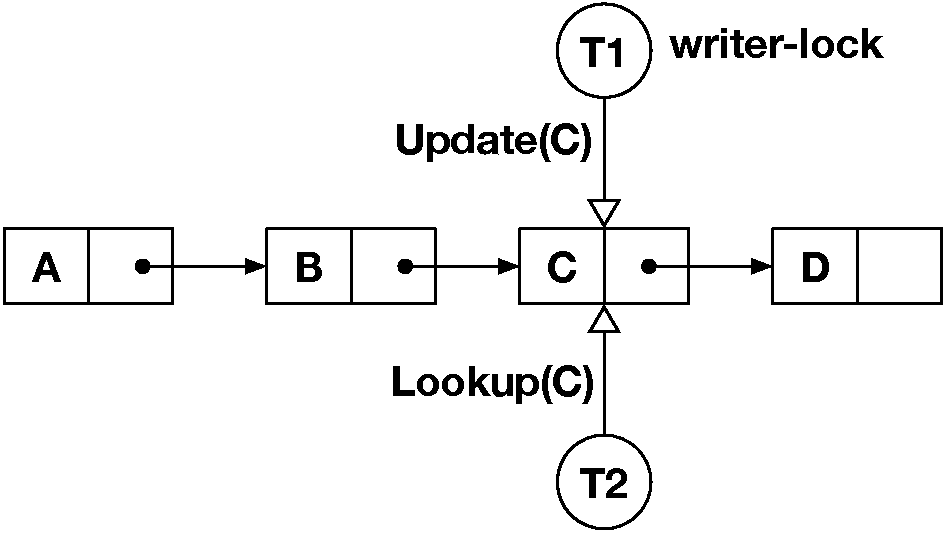
\includegraphics[width=0.9\textwidth]{figures/rcu_ex1}}
      \caption{Two threads access a list respectively to update and a lookup the
        node \emph{C}.}
      \label{fig:rcu_ex1}
    \end{flushleft}
  \end{minipage}
  \hfill
  \begin{minipage}[b]{0.47\textwidth}
    \begin{flushright}
      \centering
      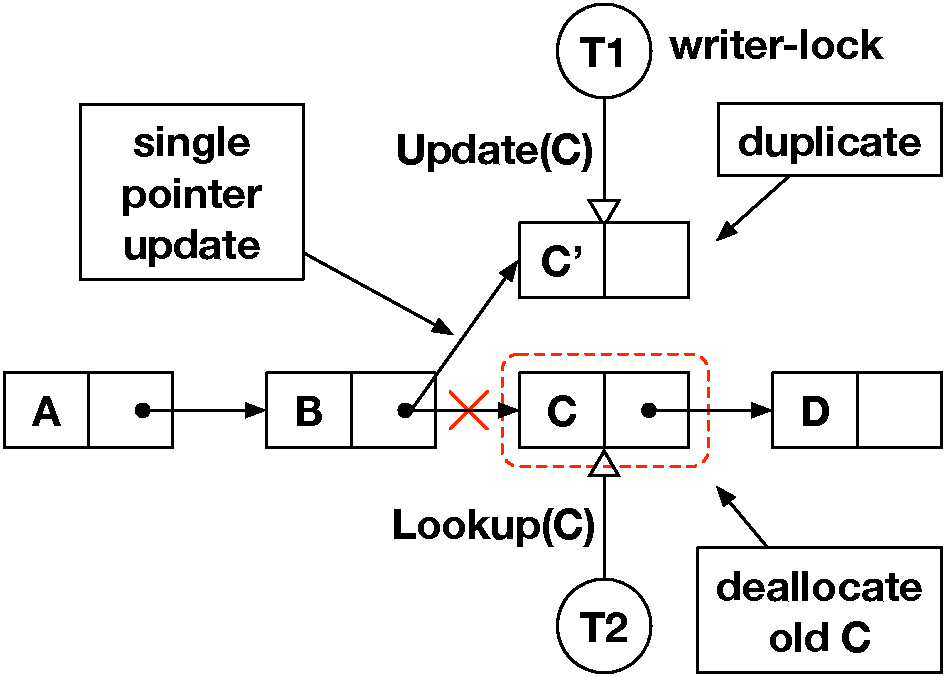
\includegraphics[width=0.9\textwidth]{figures/rcu_ex2}
      \caption{The writer \emph{T1} duplicates the node \emph{C} and performs the
        single pointer update.}
      \label{fig:rcu_ex2}
    \end{flushright}
  \end{minipage}
  \vspace{-10pt}
\end{figure}

Let us suppose that we have two threads that we want to access a linked list,
like the one in Figure~\ref{fig:rcu_ex1}.
%
The thread \emph{T1} wants to update the node \emph{C} while the thread
\emph{T2} concurrently wants to lookup for the node \emph{C}.
%
We then have a conflict between the two threads.
%
The thread \emph{T1} acquires a \emph{write-lock} and it starts to traverse
the list, at the same time the thread \emph{T2} starts looking for the node
\emph{C} traversing the list as well.
%
Let us assume that both threads reach the node \emph{C} at the same time, as
shown in Figure~\ref{fig:rcu_ex1}.
%
In order to avoid conflict, the thread \emph{T1} duplicates the node \emph{C}
(to \emph{C'}) and performs a single pointer update making \emph{C'} reachable
and \emph{C} unreachable, as illustrated in Figure~\ref{fig:rcu_ex2}.
%
The final operation consists in deallocating the old node \emph{C}.
%
Prior to deleting the node \emph{C}, the thread \emph{T1} needs to make sure
that no other threads are still reading it.
%
For this purpose, it waits for a \emph{grace period}, a time interval after
which it is safe to deallocate the object.

This example shows how RCU is able to perform a single pointer update.
%
However, applying RCU to more complex data structures or operations may result
in a less straightforward pointers update.
%
Let us suppose to have a linked list where a thread \emph{T1} wants to update
all the even nodes, as shown in Figure~\ref{fig:rcu_ex3}.
%
Thread \emph{T1} duplicates the node that it wants to update, and then it
needs to update their pointers.
%
With a single pointer update it is impossible to update both pointers at the
same time.
%
Therefore, thread \emph{T1}, for instance, updates first the pointer to the
node \emph{B'}.
%
If at the same time another thread \emph{T2} (Figure~\ref{fig:rcu_ex4}) tries
to lookup for all the even nodes, it will see an inconsistent mix of states
that would not happen in any serial execution on this data structure.
%
In order to find a solution to this problem, programmers must be able to see
this kind of race conditions and solve them manually using some
synchronization mechanism.
%
However, with more complex data structures (e.g.\ search tree, graph) solving
these race conditions may prove very difficult.

\begin{figure}
  \begin{minipage}[t]{0.47\textwidth}
    \begin{flushleft}
      \centering
      \raisebox{0pt}{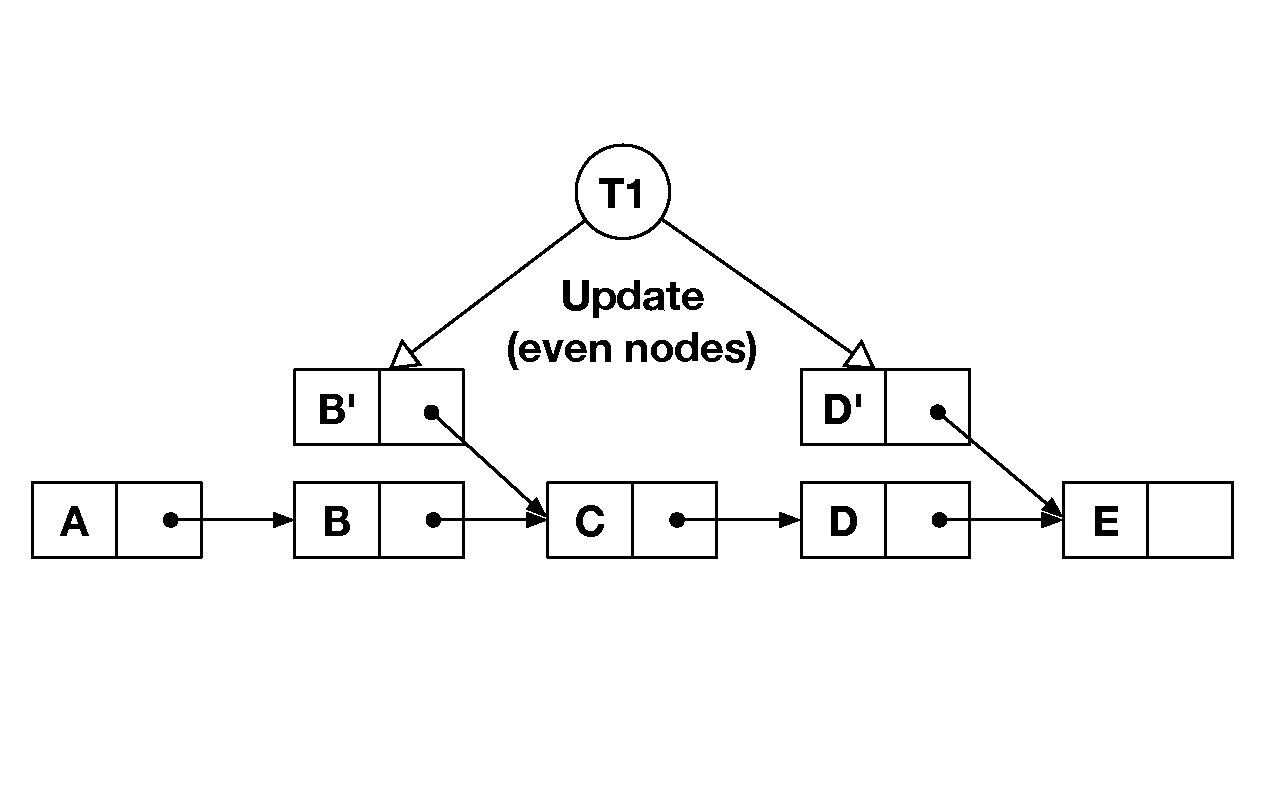
\includegraphics[width=1.0\textwidth]{figures/rcu_ex3}}
      \caption{Thread \emph{T1} wants to update all the even nodes. It
        traverses the list and create a duplicates for each node it wants to
        update.}
      \label{fig:rcu_ex3}
    \end{flushleft}
  \end{minipage}
  \hfill
  \begin{minipage}[t]{0.47\textwidth}
    \begin{flushright}
      \centering
      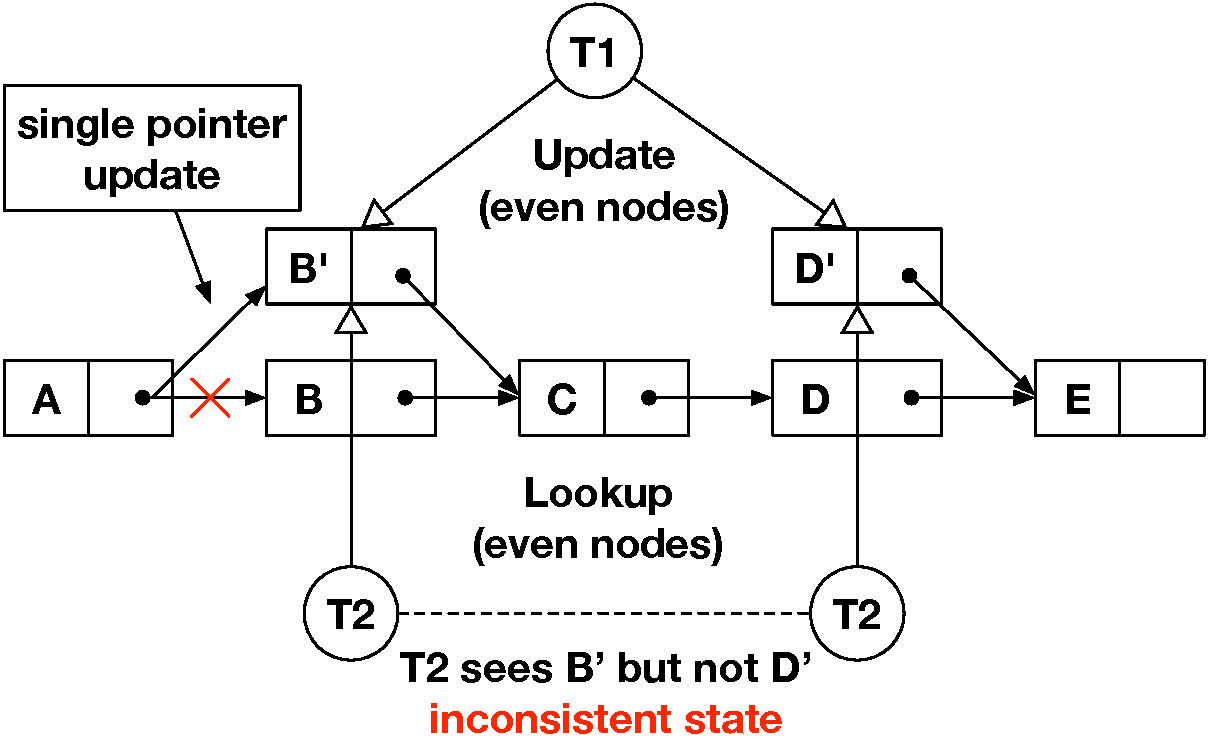
\includegraphics[width=1.0\textwidth]{figures/rcu_ex4}
      \caption{A second thread \emph{T2} wants to lookup for all the even
        nodes. RCU allows only single pointer updates, \emph{T1} cannot update
        the pointers to \emph{B'} and \emph{D'} simultaneously, so the thread
        \emph{T2} will see an inconsistent state.}
      \label{fig:rcu_ex4}
    \end{flushright}
  \end{minipage}
  \vspace{-5pt}
\end{figure}

\subsubsection*{RLU Description}
\label{sec:member412}
As stated above, RLU is an extension to RCU that provides both unsynchronized
traversal and multi-location atomic updates, simplifying the work of the
programmer but still guaranteeing efficiency and performance.
%
RLU allows multiple object updates in a single operation by combining RCU
mechanism with a global clock (inspired by TM mechanisms) and per-thread
object-level logs.

Specifically, RLU maintains different information (metadata) as global,
\mbox{per-thread} and \mbox{per-object}:

\paragraph{Global:} The only global information maintained by RLU are the
global clock, and a global array of threads used to determine the currently
active threads.

\vspace{-10pt}
\paragraph{Per-Thread:} Each thread maintains:

\begin{itemize}
\item two \emph{write-logs}: hold new object copies, each object in the
  write-log has a header that holds information such as: thread id, pointer to
  the actual object in memory, object size.
\item \emph{local clock} (\emph{l-clock}) and \emph{write clock}
  (\emph{w-clock}): control the write-log stealing mechanism of threads.
\item \emph{run counter}: indicates when the thread is active.
\end{itemize}

\vspace{-10pt}
\paragraph{Per-Object:} RLU attaches to each object a header which contains a
pointer to the copy of the object in a write-log (\emph{malloc()} calls are
hooked with a call to a \emph{rlu\_alloc()} function that attaches the header
at the object allocation time).
%
When there is no copy the pointer is \emph{NULL}.
%
RLU API provides specific macros and functions to access and modify the
metadata headers of an object.
\\

\noindent
The RLU algorithm works approximately in the following way:

\begin{itemize}
\item When an operation starts (read or write), it always reads the global
  clock first.
\item Each write operation that wants to modify a shared object, first copies
  the object in a per thread write-log and modifies the copy.
\item A write operation locks the object at its first modification (and
  duplication) in order to avoid conflicts with concurrent writes.
\item Each thread maintains a local clock (\emph{l-lock}) that reflects the
  value of the global clock (\emph{g-lock}), and a write clock
  (\emph{w-clock}, initially initialized to $\infty$) that is used by a thread
  to determine whether it needs to steal a new object copy (from a writing
  thread) or can read it from memory.
  %
  Therefore, when a thread wants to read an object:
  \begin{itemize}
  \item If it is not locked (by a thread $T_w$ performing a write operation)
    reads it from memory.
  \item If it is locked:
    \begin{itemize}
    \item If \emph{l-clock} $\geq T_w$.\emph{w-clock} steals the new copy from $T_w$.
    \item Read the object from memory, otherwise.
    \end{itemize}
  \end{itemize}
\item To commit the new object copies, a write operation computes the new
  clock value and stores it into the \emph{w-clock}, \emph{l-clock}, and
  \emph{g-clock} in this order.
  %
  The update of the clock divides the operations into two categories:
  \begin{itemize}
  \item \emph{old operations}, those that started before the clock update.
    %
    These operations will read the old object copies.
  \item \emph{new operations}, those that started after the clock update.
    %
    These operations will read the new object copies from the writer.
  \end{itemize}
  %
  The writer waits until \emph{old operations} have finished (\emph{grace
    period}, this wait is implemented by calling the \emph{RLU\_SYNCHRONIZE}
  function), and then it can safely overwrite the old objects in memory with
  the new objects from the writer-log.
  %
  It releases the locks.
  \item The basic algorithm does not provide write--write synchronization which must
    be managed by the programmer.
    %
    An easy approach to synchronize multiple write operations is to execute them
    serially.
\end{itemize}

% RLU provides a simple synchronization mechanism that is comparable and
% sometimes better in terms of performance than RCU and it simplify programmers
% work presence of race conditions.

\paragraph{Example:}

\begin{figure}[t]
  \begin{minipage}[b]{0.47\textwidth}
    \begin{flushleft}
      \centering
      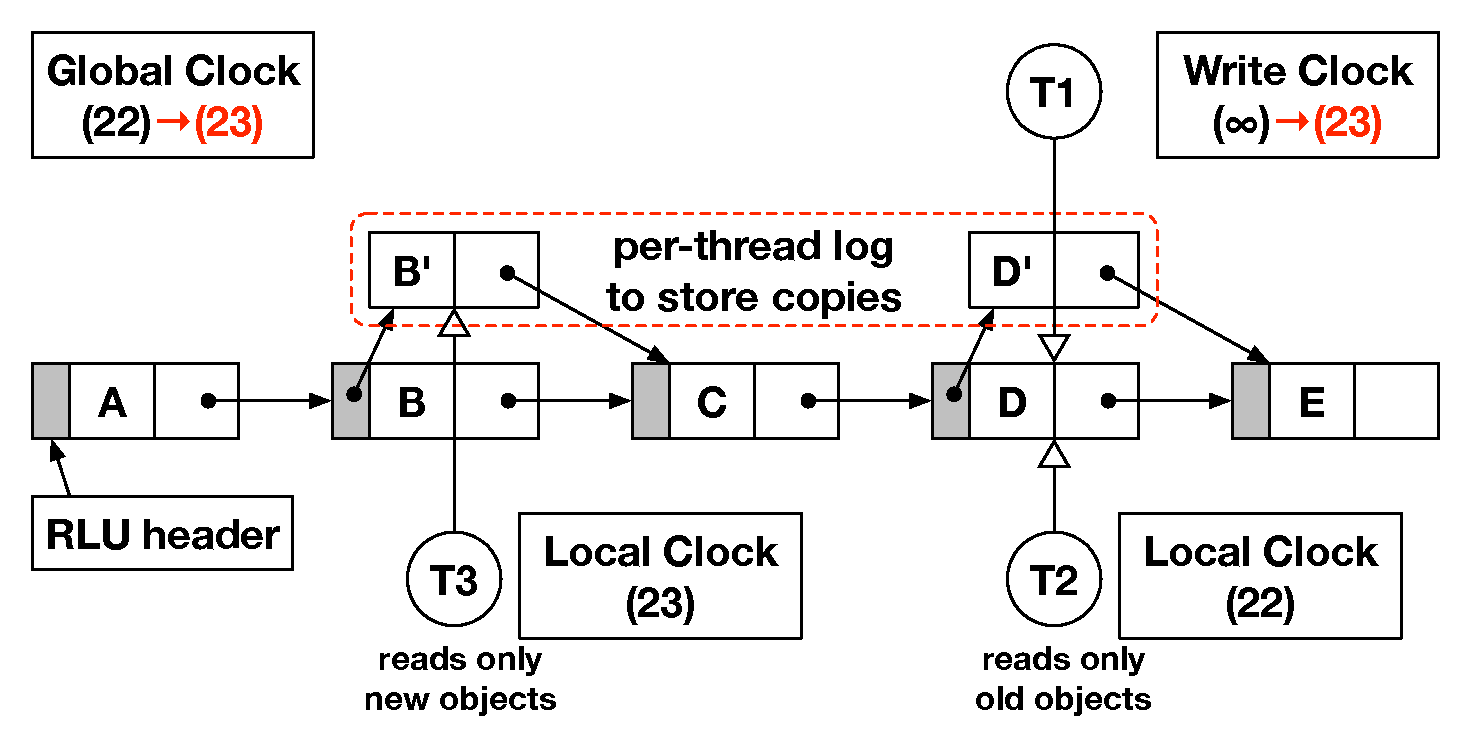
\includegraphics[width=1.0\textwidth]{figures/rlu_ex1}
      \caption{Thread $T1$ copies the object ``B'' and ``D'' in the per-thread
        write-log, updates the values and start the commit procedure by
        updating the clocks (in red). Thread $T2$ (that started the operation
        before the commit) reads the object ``D'' from the memory, while
        thread $T3$ (that started the operation before the commit) reads the
        object ``B'' from the $T1$'s per-thread write-log.}
      \label{fig:rlu_ex1}
    \end{flushleft}
  \end{minipage}
  \hfill
  \begin{minipage}[b]{0.47\textwidth}
    \begin{flushright}
      \centering
      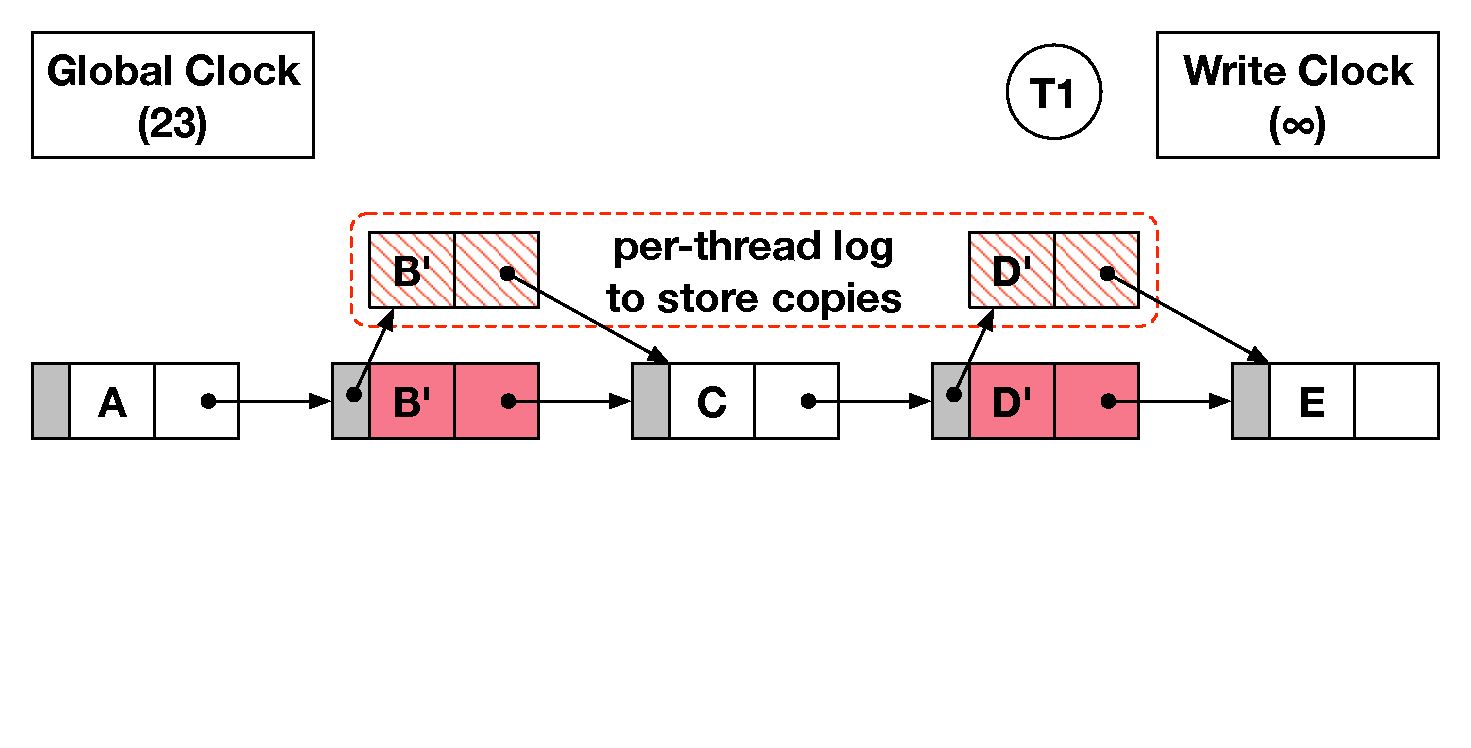
\includegraphics[width=1.0\textwidth]{figures/rlu_ex2}
      \caption{Thread $T1$ writes the modification in memory, swaps the log
        and reset the write-clock to $\infty$. \textcolor{white}{empty empty
          empty empty empty empty empty empty empty empty empty empty empty
          empty empty empty empty empty empty empty empty empty empty empty
          empty empty empty empty empty empty empty empty empty empty empty}}
      \label{fig:rlu_ex2}
    \end{flushright}
  \end{minipage}
  \vspace{-10pt}
\end{figure}

Figure~\ref{fig:rlu_ex1} and Figure~\ref{fig:rlu_ex2} show an example of RLU
algorithm.
%
Each object has a header that contains the pointer to the object copy in the
write-log of a thread, initially the pointer is \emph{NULL}.
%
When a thread $T1$ wants to modify some objects (e.g.\ nodes $B,D$), it first
tries to lock the objects, and if successful, generates the copies, storing
them in the per-thread write-log.
%
A second thread $T2$ that wants to read an object, first updates its local
clock to the value of the global clock.
%
The local clock is used by the reading thread to decide if it has to read the
real object from memory or the copy of the object from some per-thread
write-log.
%
The writer instead has a write clock which is initialized to $\infty$.
%
Whenever $T1$ wants to commit its modifications, it first updates the clocks:
write clock and global clock to the next value (from $22$ to $23$ in
Figure~\ref{fig:rlu_ex1}).
%
At this point, the old copies are reachable by the threads that started
reading the objects before the global clock update, while the new copies are
reachable by the thread that started after the global clock update.
%
Thread $T2$ will keep seeing the old copies, while $T3$ will see the new
copies, as in Figure~\ref{fig:rlu_ex1}.
%
The threads make a simple check, whenever their \emph{l-clock}
$\geq T_w$.\emph{w-clock} they steal the new copy from the per-thread
write-log of the writing thread, otherwise they read the old object from
memory.
%
In this case it is impossible for the threads to read a mix of state, as
happened in RCU, they will see either all the new object or all the old
objects.
%
In the next step of the commit $T1$ wait for the \emph{grace period} (calling
\emph{RLU\_SYNCHRONIZE}), to wait for the old reading threads ($T2$) to
finish.
%
When thread $T2$ is done, $T1$ writes the new objects back to memory
(Figure~\ref{fig:rlu_ex2}), resets the write clock to $\infty$, and unlock the
object.
%
It is important to notice that, it is necessary to wait for another
\emph{grace period} before clearing the current write-log and reusing it.
%
The reason for this is that it may still be used by threads that stole the
copies from this write-log.
%
Therefore, the writing thread, as a last operation of the commit, swaps the
\emph{current write-log} with a \emph{new write-log} (remember each thread has
two write-log available), and waits for the completion of the next
\emph{RLU\_SYNCHRONIZE} to swap again the logs and reuse safely the
\emph{current write-log}.

\subsection*{Explain the problem that RLU Deferring (Section 3.7) solves and
  give a pathological example scenario where RCU’s ``synchronize'' operation
  would have high overheads but RLU Deferral would not.}
\label{sec:member42}
\vspace{-5pt}
The RLU experiments show that when operations are short and fast, the
algorithm performance decreases significantly.
%
This is because every time a writer has to perform a write, it calls the
\emph{RLU\_SYNCHRONIZE} function, which implements the wait of the \emph{grace
  period} that a writer has to let pass to safely write the updated objects
back to memory.
%
The \emph{RLU\_SYNCHRONIZE} calls introduces a high overhead, i.e.\ for each
small write operation the writer has to wait the \emph{grace period}.
%
In order to solve this performance problem, the authors introduce a variant to
RLU called \emph{RLU Deferring}, that indeed defers (or delays) the call to
the \emph{RLU\_SYNCHRONIZE} as much as possible -- making this call only if
strictly necessary.

RLU Deferring works in the following way.
%
At each commit phase, after the writer stores the current write-log, it
generates a new one for the next write operation.
%
This allows to keep performing write operations without blocking until a
different thread needs to update an object that is already locked.
%
Only at this moment, the new writer issues a ``sync request'' to the writer
thread that is holding the lock in order to force it release the lock.
%
Therefore, the writer thread performs the normal operations: increment global
clock, execute the \emph{RLU\_SYNCHRONIZE} call, write the objects to memory
and finally unlock.

RLU Deferring introduces significant advantages in terms of performance, since
it heavily limits the number of actual write--write conflicts.
%
It also reduces the global clock updates, which as a consequence delays the
stealing process, allowing threads to read from memory (instead from a thread
write-log), and experience less or none cache misses (higher in number when
the memory is updated more often).
\\

An example that would show the advantages of RLU Deferring compared to RCU is
given by a benchmark where multiple threads perform a high rate of updates on
a linked-list while other threads read the same objects.
%
In RCU, when a thread updates an object, it has to commit (since it only
performs single-pointer updates), and let the \emph{grace period} pass prior
to starting the next write operation.
%
This is to wait for the reading threads to terminate their operations.

In RLU Deferring, the call to \emph{RLU\_SYNCHRONIZE} happens only when a
write--write conflict manifests.
%
In this case, the current writing thread receives the ``sync request'' from a
new writer, and it has to perform the commit and call the synchronize
function.
%
If no write--write conflict happens, the writing threads can keep updating the
objects while the reading threads access the copies.
%
RLU Deferring waits for a smaller number of \emph{grace periods} than RCU,
reducing the runtime overhead.

In general, increasing the number of writers (and so write--write conflicts)
RCU introduces a sequential bottleneck, while RLU Deferral can perform
concurrently the write operations increasing the scalability.
%
The authors in Figure~10 of~\cite{Matveev:2015:RLS:2815400.2815406} show the
best performance of RLU compared to RCU, increasing the updates rates on a
linked-list.
%
This should reinforce the fact that RLU Deferral (which is faster than RLU)
have less overheads than RCU, as described in the previous example.

However, the experimental results show that this optimization is more
significant for a high number of cores ($>20$).
%
Therefore, a better example that shows the performance boost of the deferring
approach is the benchmark on Citrus Tree on a 80 cores machine.
%
Indeed, the performance results show that for an high threads count RLU
Deferral is faster than RCU by a factor of two.
%
This is because RCU has to execute the synchronization call for each delete,
while RLU Deferral calls the synchronization function only on actual
write--write conflicts.

\subsection*{Can RLU Deferral result in linearizability violations?}
\label{sec:member43}
\vspace{-5pt}
RLU Deferral can not result in linearizability violations, because it
guarantees that when a thread commits a write operation all the other threads
that started later than the commit operation will see the value of that write.
%
When a thread performs a commit it first increments the global clock,
which splits the concurrent threads operations in \emph{old operations} and
\emph{new operations}.
%
The old operations are those ones that started before the clock updates, so
these threads will read the old value of the objects thanks to the
per-thread write-log that contains the copies.
%
Furthermore, the new operations that started after the clock update will read
the new values from the new per-thread write-log (via stealing).
%
The threads can make this decision by first reading the global clock and
comparing it with the writing thread write clock.
%
This allows a thread to ``understand'' if they started an operation before or
after the commit and so they should read the new or the old value.
%
If a write--write conflict happens, the writing thread receives a ``sync
request'' and besides executing the commit it also calls the
\emph{RLU\_SYNCHRONIZE}, that makes the writing thread wait for the \emph{old
  operations} to finish, prior to writing the updates on memory.
%
As the commit updated the global clock the new write operation will now see
the new value.
%
This guarantees that each thread is always able to see a consistent memory
state (that could happened in some serial execution) which existed at the
global time when it started the operation.

\subsection*{Does code using RLU Deferral in 3.7 meet the definition of being
  ``lock-free''?}
\label{sec:member44}

\vspace{-5pt}
Considering the definition of lock-free
in~\cite{Herlihy:2008:AMP:1734069}~\footnote{A method is lock-free if it
  guarantees that infinitely often some method call finishes in a finite
  number of steps.
  %
  Let us also consider some larger ADT lock-free if and only if all of the
  operations/methods on it are lock-free.}.
%
A code using RLU Deferral can be considered lock-free for read operations and
non lock-free for write operations.

\begin{itemize}
\item \emph{Read Operations}: Read operations are lock-free because a reading
  thread can always make progress and there is nothing that can stop them from
  proceeding.
  %
  A reading thread can always decide, based on the values of the global clock
  and the writer clock, to read an object from the memory (old value) or from
  a thread write-log (new value).
\item \emph{Write Operations}: Write operations are non lock-free because
  there exists a situation where a new writer may be stopped by another writer
  that fails to respond to a ``sync request''.
  %
  In such circumstances the current writer never completes the commit
  operation and never calls the synchronize function, preventing the new
  writer to start its operations, thus none of the threads finish their
  operation in a finite number of steps.
\end{itemize}

\vspace{-10pt}
\printbibliography

\end{refsection}

%%% Local Variables:
%%% mode: latex
%%% eval: (flyspell-mode 1)
%%% TeX-master: "root.tex"
%%% End:


\end{document}

%%% Local Variables:
%%% mode: latex
%%% eval: (flyspell-mode 1)
%%% TeX-master: "root.tex"
%%% End:
